\documentclass[12pt]{report}
\usepackage[english]{babel}
\usepackage{natbib}
\usepackage{url}
\usepackage[utf8x]{inputenc}
\usepackage{amsmath}
\usepackage{graphicx}
\graphicspath{{images/}}
\usepackage{parskip}
\usepackage{fancyhdr}
\usepackage{vmargin}
\usepackage{colortbl}
\usepackage{hyperref}
 \usepackage{listings}
 \lstset{
 keywordstyle=\color{blue},
 language=java
}
\setmarginsrb{3 cm}{2.5 cm}{3 cm}{2.5 cm}{1 cm}{1.5 cm}{1 cm}{1.5 cm}

\author{SOW Sokhna Maimouna} % Author

\makeatletter
\let\theauthor\@author
\renewcommand{\thesection}{\@arabic\c@section}


\makeatother

\pagestyle{fancy}
\fancyhf{}
\lhead{\theauthor}
\rhead{\rightmark}
\lfoot{Universite Paris Nanterre}
%\rfoot{Cosmo Consult}
\cfoot{\thepage}
\renewcommand{\footrulewidth}{0.4pt}%trait horizontal pour le pied de page

\begin{document}

%%%%%%%%%%%%%%%%%%
%%% First page %%%
%%%%%%%%%%%%%%%%%%

\begin{titlepage}
\begin{center}


\includegraphics[width=0.6\textwidth]{fac}\\[1cm]

{\large\textbf{ M}éthodes \textbf{I}nformatiques \textbf{A}ppliquées à la \textbf{G}estion des \textbf{E}ntreprises}\\[0.8cm]


{\large \textbf{Mémoire Master 2 Classique}}\\[0.5cm]

\vfill

% Title
\rule{\linewidth}{0.5mm} \\[0.4cm]
{ \huge \bfseries Comment intégrer les blockchains dans les transactions bancaires ?  \\[0.4cm] }
\rule{\linewidth}{0.5mm} \\[1.5cm]

\vfill

% Author and supervisor
\noindent
\begin{minipage}{0.5\textwidth}
  \begin{flushleft} \large
    \emph{Auteur :}\\
   Sokhna Maimouna \textsc{SOW}\\
  \end{flushleft}
\end{minipage}%
\begin{minipage}{0.5\textwidth}
  \begin{flushright} \large
    \emph{Encadrant :} \\
   Mme Marie-Pierre \textsc{Gervais}\\
  \end{flushright}
\end{minipage}

\vfill

% Bottom of the page
{\large Année scolaire \\ 2017 - 2018}

\end{center}
\end{titlepage}

%page de garde
\thispagestyle{empty}
\newpage
~

\newpage
\section{Remerciements}

\hspace{1cm} Je puise une profonde gratitude au fin fond de  mon coeur pour l'envoyer vers des personnes spéciales, particulièrement vers mon père \textbf{Ibrahima Sow}, un père qui s'est sacrifié pour que ses enfants réussissent dans leurs études. "\textbf{les études avant tout}",ça a toujours été ta conviction. Un père qui nous a mis dans les meilleures conditions possibles. Un père qui a transmis à ses enfants les bonnes valeurs. Un père qui nous a donné une éducation, "DURE et COMPLIQUÉE",mais qui a fait de moi ce que je suis aujourd'hui. Je ne saurais te remercier assez, papa, mais sache que tu occupes les \textbf{3/4} de mon coeur.\\

\hspace{1cm} Merci \textbf{mère Ngane}, la meilleure des mamans. Celle que je n'échangerais pour rien au monde. Celle qui peut mourir de faim afin que ses enfants puissent avoir le ventre plein. Celle qui nous a toujours protégé contre tout et tout le monde. Celle qui n'a jamais accepté qu'on ait un visage triste. Celle qui a un coeur en or. Je te remercie du fond du coeur maman, une goutte de larme pleine de bonheur et de reconnaissance m'échappe à chaque fois que je pense profondément à toi.\\

\hspace{1cm} Je dis un grand merci à ma grande soeur \textbf{Coumba} qui est comme une 2ème mère. Tu m'a prise sous ton aile depuis que je suis en France et grâce à toi je ne manque de rien. Merci à mon grand frère \textbf{Amar},pour tout ce que tu as fait pour moi et à mon grand frère \textbf{Moussa} aussi. Un grand merci à mon homme, \textbf{Abou}, qui m'a toujours soutenue et qui essuie mes larmes dans les moments difficiles.\\

\hspace{1cm} je vous remercie, vous mes enseignants pour tout le savoir que vous m'avez transmis durant tout mon cursus scolaire. Je ne saurais vous rendre la pareille. Merci à ma tutrice \textbf{Mme  Marie-Pierre Gervais} pour sa compréhension et tous ses conseils durant l'élaboration de ce mémoire. Merci aussi à mon tuteur d'entreprise,une personne que j'ai découverte il y a peu mais que j'apprécie déjà, \textbf{David Granzotto} pour sa disponibilité et sa précieuse aide sur le choix de mon sujet.\\ 

\hspace{1cm} Et enfin merci à toutes les personnes qui ont toujours été présentes pour moi. Surtout à mes camarades de classe qui m'ont toujours encouragée et ont rempli de gaieté mes journées. Je ne saurais terminer sans remercier \textbf{Minh Huy LE}, qui m'a beaucoup aidé durant toute l'année scolaire. \\

  \begin{flushright} \large
    \emph{MERCI A VOUS TOUS DU FOND DU COEUR !} \\
  \end{flushright}


%%%%%%%%%%%%%%%%%%%%%%%%%%%%%%%%%%%%%%%%%%%%%%%%%%%%%%%%%%%%%%%%%%%%%%%%%%%%%%%%%%%%%%%%%
\newpage
\renewcommand{\contentsname}{Table des matières}
\tableofcontents
\pagebreak

%%%%%%%%%%%%%%%%%%%%%%%%%%%%%%%%%%%%%%%%%%%%%%%%%%%%%%%%%%%%%%%%%%%%%%%%%%%%%%%%%%%%%%%%%

\section{Introduction}
\hspace{1cm} Notre monde évolue au rythme des innovations et des nouvelles technologies. Aujourd'hui, nous sommes témoins d'une nouvelle révolution mondiale avec une portée assez difficile à mesurer mais mettant en avance des possibilités d'applications infinies. Cette révolution est marquée par le phénomène "\textbf{blockchain}". Elle est née du croisement d'une technologie cryptographique de pointe basée sur les registres distribués et d'un contexte sociologique opportun. Le cas de la blockchain est juste \textit{phénoménal}. En effet la rapidité de son développement technologique coïncide avec un contexte sociologique favorable, ce qui augmente les chances de tirer profit des grandes innovations technologiques en les transformant en un vrai usage. \\

\hspace{1cm} Derrière ce concept de blockchain se cachent les cryptomonnaies qui se \\démarquent des monnaies traditionnelles sur différents plans. Non seulement elles sont dématérialisées, anonymes, sécurisées mais ces devises peuvent s'échanger entre elles et permettent de faire des transactions bancaires. Et pendant ce temps, nous avons un système bancaire avec un réseau trop organisé, encadré et centralisé qui est bien construit et trop hiérarchisé avec des dirigeants qui contrôlent tout le système et ont toujours le dernier mot.\\

\hspace{1cm} Face à cette situation, il me semble opportun de s'interroger sur la performance et l'avenir des banques. Puisque c'est assez difficile de contourner les banques, cela me pousse à chercher comment procéder à mettre en place les blockchains afin de faciliter le monde monétaire de demain. Comment intégrer les blockchains dans les transactions bancaires ? Quels sont les acteurs à impliquer ? Tellement de questions qui me motivent à faire une étude approfondie et dans la mesure du possible trouver une solution pour faire cohabiter les banques et les blockchains.\\

\hspace{1cm} A travers ces lignes je vais d'abord expliquer ce que c'est la blockchain en partant de sa création jusqu'à son processus final en détaillant son architecture et voir les différentes blockchains qui existent de nos jours. Ensuite j'étudierais l'impact des blockchains dans l'actualité économique, plus particulièrement dans les transferts d'argent, en créant d'abord ma propre blockchain à appliquer sur ces transferts et parler brièvement de certains autres transactions. Et pour finir je mettrais en évidence les faiblesses de cette nouvelle technologique, qui n'est pas sans faille.


%%%%%%%%%%%%%% Glossaire %%%%%%%%%%%%%%
\newpage
\section{Glossaire}
\begin{tabular}{|c|c|}
\hline 
\rowcolor{green}KEY & Value \\

\hline
Subprimes & Prêts immobiliers accordées aux américains ne remplissant \\ & pas les conditions pour un prêt classique \\ 

\hline 
BTC & Symbole utilisé pour représenter l'unité de compte du bitcoin \\

\hline
Cyber-marchand & Commerçant proposant ses services via un site de e-commerce \\

\hline
FEVAD & Fédération du e-commerce et de la vente à distance\\

\hline
TPE & Terminal de paiement électronique\\

\hline
Coin & Terme utilisé pour désigner les monnaies bitcoin\\

\hline
GBP & Code qui signifie : livre sterling, la monnaie du Royaume-Uni\\

\hline
USD & United States dollar, code de la monnaie des États-Unis \\

\hline
EUR & Code qui désigne : Euro, la monnaie européenne \\

\hline
QR & Acronyme de Quick Response et qui est un,code barre 2D\\

\hline
IBM & International Business Machines Corporation, est une société \\ & multinationale américaine\\

\hline
C2C & Consumer to Consumer, regroupe les activités entre consommateurs\\  

\hline
P2P & Peer-to-Peer, modèle de réseau où chaque client est aussi un serveur\\

\hline
B2B & Business to Business, entreprise qui vise une clientèle d'entreprises\\

\hline
B2C & Business to Consumer, entreprise qui vise une clientèle de consommateurs\\

\hline
UE & Union Européenne \\

\hline
REQ & Request Network, plate-forme de cryptomonnaie\\

\hline
Spreads & Différentiel entre deux taux\\

\hline
UTXO & Sortie non dépensée des transactions bitcoin\\

\hline 
\end{tabular} 

\newpage
\section{Fonctionnement de la blockchain}

%%%%%%%%%%%%%% Historique %%%%%%%%%%%%%%

  \subsection{Historique}
\hspace{1cm} Tout a commencé par un groupe de 'geek' auto-organisé, sans hiérarchie et sans État qu'on appelle des \textbf{crypto-anarchistes}. Ces crypto-anarchistes savaient coder les données de façon à ce que personne d'autre que le destinataire ne puisse les déchiffrer. Ils se sont mis à "crypter des monnaies" d'où la naissance des \textbf{cryptomonnaies} appelées aussi \textbf{ monnaies virtuelles}. Si ces cryptomonnaies remontent aux années 70, ce phénomène devient célèbre qu'en début de 2009 avec la création de la blockchain et du bitcoin.\\

\hspace{1cm} En effet vers 2008, il y a eu une crise financière des subprimes. Les banques déclenchent alors la planche à billet afin de créer des euros et des dollars pour maintenir le système bancaire à flots. Et c'est vers cette même période précise qu'un certain \textbf{Satoshi Nakamoto}, un pseudo qui lui est attribué, publie un livre blanc de 10 pages, dans un forum de discussion, appelé \textbf{\textit{Bitcoin - A Per to Per Electonic Cash System }} qui va révolutionner le monde monétaire. Par la suite, plusieurs personnes ont prétendu être Nakamoto mais nous n'avons jamais pu découvrir le vrai cerveau qui se cachait derrière. Il est resté actif jusqu'à mi 2010 pour ensuite disparaître des radars avec une fortune estimée à \textbf{980.000 token} soit \textbf{5.473.465.943 euros}. C'est ainsi qu'on assiste à la naissance  de la première monnaie virtuelle décentralisée, qui fonctionne principalement avec la blockchain. \\ 

\hspace{1cm} De ce fait la première blockchain est apparue avec la monnaie numérique bitcoin. Aussitôt le marché virtuel se met à utiliser la technologie de la blockchain et plusieurs activités ont tourné autour de cette technologie naissante. Des plate-formes, des sites Internet et même des applications ont été mis en place pour la gestion des monnaies virtuelles et une utilisation permanente des blockchains.


%%%%%%%%%%%%%% Archi %%%%%%%%%%%%%%

\newpage
  \subsection{Architecture de la blockchain}

\hspace{1cm} Qu'est que la blockchain? Certains diront que c'est juste une écriture comptable d'opérations numériques qui sont partagées entre de multiples parties prenantes. D'autres diront que c'est un ensemble de réseau maillé d'ordinateurs reliés entre eux. Tellement de définitions lui sont attribuées. Mais quand est-il réellement de ce nouveau fléau? Comment est elle structurée? Quelles sont ses composantes? Essayons plutôt d'expliquer le mécanisme de la blockchain pour en sortir une définition adéquate.

\hspace{1cm} Prenons un livre où nous allons écrire toutes les dépenses que chacun a réalisé avec les montants et les dates.

\begin{itemize}
    \item Le 01/08/2009 à 16h : Alice paie 250 euros à Bob 
    \item Le 03/08/2009 à 20h : Bob paie 30 euros à Carole
    \item Le 03/08/2009 à 22h : Alice paie 15 euros  à Carole
    \item Le 04/08/2009 à 19h : Carole paie 20 euros  à Clara
    \item etc.
\end{itemize}

\begin{center}
    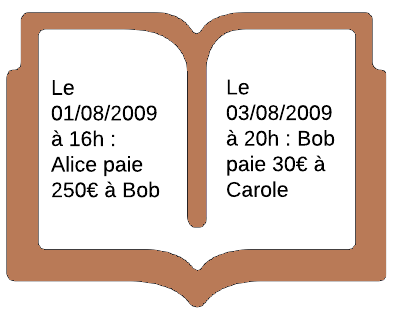
\includegraphics[width=0.5\textwidth]{livre_compte}

    \textbf{\underline{Livre de compte}} \\[1cm]
\end{center}

Nous avons ici un grand livre qui dit qui a payé qui. Il n'est dit nulle part de combien d'argent vous disposez, mais nous le savons bien car nous avons toutes les échanges, leurs détails et le contenu du compte initial, donc il suffit juste de faire ses déductions. Par contre nous pouvons avoir des centaines d'échanges alors que le nombre de ligne d'un livre est limité. Comment faire dans ce genre de cas alors? C'est très simple il faut prendre un nouveau livre et continuer à remplir. Et pour ne pas se perdre les livres sont numérotés. Chaque livre contient le résumé du précédent, ce qui permet de les relier entre eux et d'avoir une continuité. Nous obtenons ainsi un enchaînement de livres remplis de toutes les échanges.\\

\begin{center}
    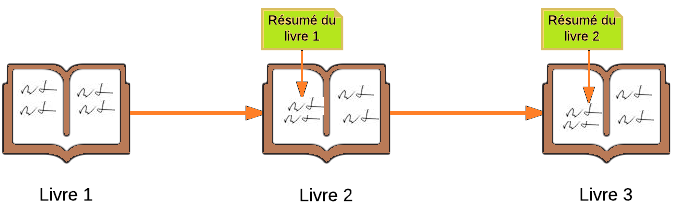
\includegraphics[width=1\textwidth]{livre_compte_2}

    \textbf{\underline{Enchaînement des livres}} \\[1cm]
\end{center}

\hspace{1cm} Et dans le monde de la cryptomonnaie, à la place de ces livres, nous avons des fichiers appelés \textbf{blocs}. Ces blocs sont construits les uns à la suite des autres, formant ainsi une \textbf{chaîne de blocs}. D'où le nom de \textbf{Blockchain}.\\

\hspace{1cm} \textbf{Mais comment est ce possible de résumer toutes les informations du bloc précédent dans le bloc suivant}? C'est aussi simple que complexe. La première étape est de mettre en place la structure d'un bloc qui est principalement composée de:
\begin{itemize}
    \item un index
    \item un hash qui nous permet d'identifier le bloc
    \item le hash du bloc précédent doit être trouvé dans le bloc pour préserver l'intégrité de la chaîne
    \item un timestamp pour l'horodatage 
    \item un ensemble de transactions
\end{itemize}

\begin{center}
    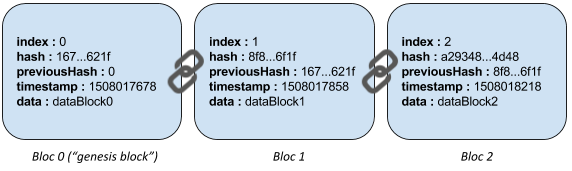
\includegraphics[width=1\textwidth]{do_bloc_1.png}

    \textbf{\underline{Enchaînement des blocks}} \\[1cm]
\end{center}

\hspace{1cm} Les \textbf{Hash} qui sont des fonctions mathématiques vont permettre de conserver l'intégrité des données en transformant n'importe quelles données en entrée en un grand nombre hexadécimal composé de lettres et de chiffres en sortie . Mais les données sont au préalablement transformées en un texte binaire avant qu'on leur applique la fonction de hachage. Il existe plusieurs fonctions de hachage. Nous pouvons en citer:
\begin{itemize}
    \item \textbf{Message Digest}, appelé aussi \textbf{MD}, comme \textbf{MD4} qui  était utilisé il y a fort longtemps dans les années 90 et abandonné au profit de \textbf{MD5} après la découverte de faiblesses dans sa conception
    \item \textbf{Les Secure Hash Function} tels que \textbf{SHA-1} qui a été longtemps utilisé et qui devrait être enterré en 2018, pour être remplacé par \textbf{SHA-2} et \textbf{SHA-3}. Ces SHA vont reprendre le contenu de chaque bloc.
\end{itemize}

\begin{center}
    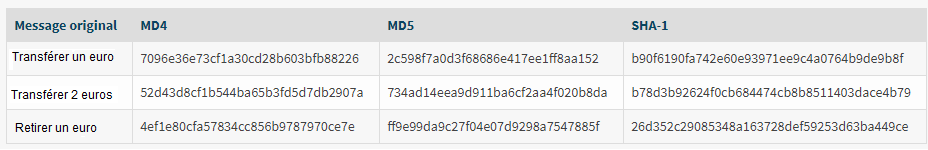
\includegraphics[width=1\textwidth]{exemple_fonction_hash.png}

    \textbf{\underline{Différentes transformations en fonction hachage}} \\[1cm]
\end{center}

Et puisque les fonctions de hachage  ne marchent que dans un seul sens, nous avons la garantie que le contenu du bloc n'a pas été changé, ce qui assure la sécurité des blockchains. Donc si vous modifiez l'historique, cela ne correspondrait plus avec le hash du 1er bloc qui est dans le 2ème bloc et ainsi de suite. \textbf{Voir annexe 1}\\

\hspace{1cm} De ce fait, en connaissant le hash du block précédent, les autres blocks suivants pourront être générés. L'ensemble de ces blocks qui forme la blockchain peut être stocker dans un tableau. Et à tout moment une chaîne de block doit être valider en terme d'intégrité. Après la validation des blockchains, la chaîne la plus longue, celle qui a le plus de block, est choisie et est mise en exécution.\\

\hspace{1cm} Derrière ce scénario, nous avons ce qu'on appelle les \textbf{noeuds} qui sont des ordinateurs reliés au réseau de la blockchain et qui utilisent un programme relayant les transactions. les noeuds sont essentiellement indispensable pour la blockchain. Non seulement ils permettent de conserver une copie du registre de la blockchain mais aussi de synchroniser et partager cette blockchain avec d’autres nœuds pour que tout le monde puisse avoir les même données. De même la particularité de la validité d'intégrité de la blockchain est toujours vraie si et seulement si de nouveaux blocks arrivent à partir d'autres noeuds et qu'il faut décider de les accepter ou pas. Par contre les noeuds suivent un certain nombre de règle :
\begin{itemize}
    \item Lorsqu'un nœud génère un nouveau block, il doit obligatoirement le diffuser sur le réseau
    \item Lorsqu'un nœud se connecte à un pair, il émet une requête pour obtenir le dernier block
    \item Lorsqu'un nœud rencontre un block qui a un plus grand index que le dernier block connu actuellement par celui-ci, il doit ajouter ce block a sa chaîne ou effectuer une requête pour obtenir la blockchain en entier
\end{itemize}

\begin{center}
    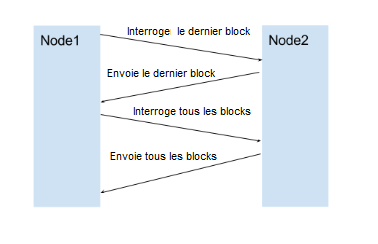
\includegraphics[width=1\textwidth]{noeud.png}

    \textbf{\underline{Synchronisation du noeud 1 avec le noeud 2 après connexion}} \\[1cm]
\end{center}


\begin{center}
    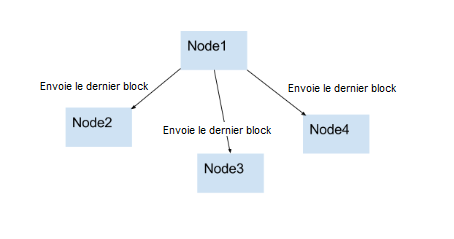
\includegraphics[width=1\textwidth]{noeud2.png}

    \textbf{\underline{Le noeud 1 génère un block puis envoie à tous les autres noeuds }} \\[1cm]
\end{center}

\hspace{1cm} Il est primordial de noter aussi que le nœud utilise deux serveurs web : 
\begin{itemize}
    \item Un serveur HTTP qui permet à l'utilisateur de contrôler le noeud
    \item Un serveur websocket HTTP pour permettre la communication peer-to-peer entre les noeuds
\end{itemize} 


\begin{center}
    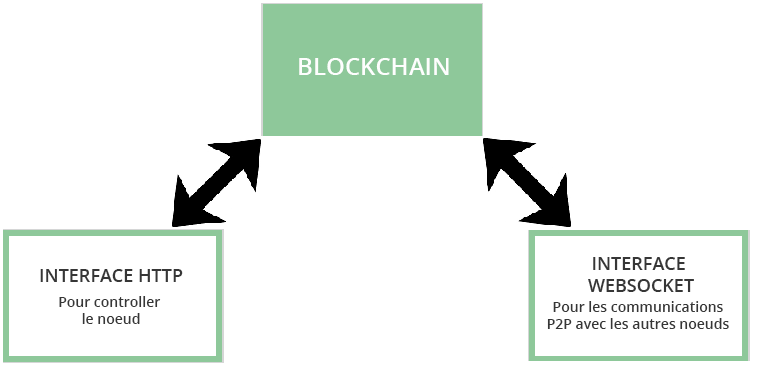
\includegraphics[width=1\textwidth]{block-noeud.png}

    \textbf{\underline{Architecture des serveurs }} \\[1cm]
\end{center}

\hspace{1cm} Nous avons ensuite ce qu'on appelle le \textbf{minage}. En effet valider les transactions dans un réseau de blockchain demande un processus très complexe. L'un des principaux système pour permettre cette validation est ce qu'on appelle le \textbf{Proof of Work}. Ce système est une sorte de puzzle à résoudre avant de pouvoir ajouter un block à une blockchain. Et c'est le fait de résoudre ce puzzle qu'on appelle \textbf{miner}. Ce \textbf{Proof of Work} permet d'éviter de tricher. Il empêche aux mineurs d'ajouter des blocs frauduleux. Le minage coûte très cher en électricité, donc si un mineur tente de tricher et qu'il était découvert, sa dépense serait perdue. Et contrairement, le fait de miner des blocks valides rapporte une grande récompense aux mineurs s'ils réussissent à résoudre le Proof of Work. Ils reçoivent la récompense sous forme de \textbf{Bitcoins}.

\begin{center}
    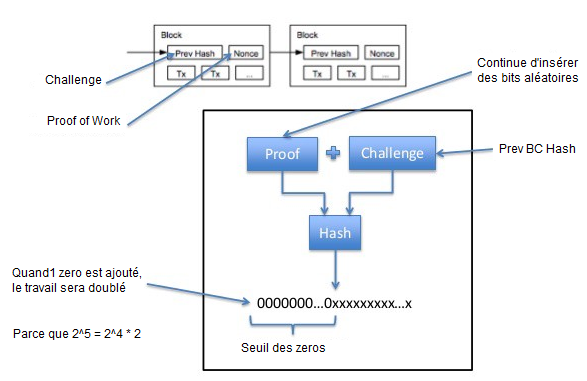
\includegraphics[width=1\textwidth]{proof.png}

    \textbf{\underline{Proof of Work}} \\[1cm]
\end{center}

\hspace{1cm} Ce concept de \textbf{minage} fait qu'il n'existe pas de banque centrale qui produit ou gère les monnaies. En effet ce sont des ordinateurs appartenant au même réseau qui font tout le travail. Ce qui fait que tout est sécurisé par le procédé cryptographique. Et c'est la difficulté pour quiconque de résoudre les preuves de calcul qui assure aussi la sécurité de toutes les transactions.\\

\hspace{1cm} Ainsi je définirais plutôt la blockchain comme une technologie de transmission d'informations et de stockage. Elle a une base de données très sécurisée et dont la gestion est traitée par un ensemble de réseau d'ordinateurs connectés entre eux et qui stockent ces données de manière distribuée. Cette base contient toute l'historique de toutes les transactions entre les utilisateurs depuis sa création et est en même temps partagée sans intermédiaire. Ce qui donne la possibilité à chaque utilisateur de vérifier la validité de la chaîne.

\begin{center}
    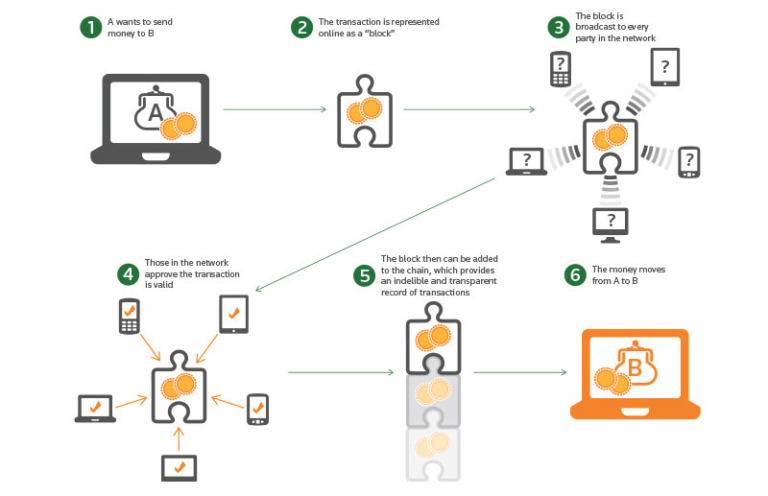
\includegraphics[width=1\textwidth]{blockchain-explained.png}

    \textbf{\underline{Processus d'une transaction dans une blockchain}} \\[1cm]
\end{center}

%%%%%%%%%%%%%% Types de blockchain %%%%%%%%%%%%%%

  \subsection{Les différents types de blockchain}
\hspace{1cm} Nous avons différents types de blockchain en fonction des secteurs. 

\begin{enumerate}

    \item \underline{\textbf{Blockchain publique}}\\ [0.3cm]
La blockchain publique est caractérisée par le fait que tous les noeuds du réseau d'échange sont contrôlés par le fameux réseau peer-peer. Pour y accéder, il y a aucune permission à demander et aucune barrière d'entrée. N'importe qui peut faire une transaction ce qui veut dire que tous les acteurs sont égaux dans leur participation du réseau. C'est le cas des monnaies virtuelles \textbf{bitcoin} et \textbf{ethereum} pour lesquels chacun a libre accès au registre et participe au même titre au processus d'approbation, celui qui permet de décider lequel des blocs doit être ajouté ou pas à la chaîne et qui définit l'état actuel du système.\\ 

\newpage
    \item \underline{\textbf{Blockchain privée}}\\[0.3cm]
la blockchain privée a son propre réseau privé dont l'accès est strictement confié au gérant qui, lui seul peut faire des modification dessus. Donc personne ne peut y accès sans y être autorisé. Cette blockchain est beaucoup utilisée par les banques grâce à sa gouvernance simplifiée, ses coûts réduits, sa rapidité, sa confidentialité surtout et du fait que les acteurs sont connus. Par contre cette blockchain perd tout son charme du moment qu'elle est privée. En effet comme l'a si bien dit \textbf{Juge David Teruzzi}, expert en bitcoin, je cite "Cette blockchain n'est pas très intéressante. Elle est certe scalable à l'infini, contrairement à la blockchain publique, mais son intérêt est limité puisqu'elle ne fait pas le lien entre différents acteurs". 

    \item \underline{\textbf{Blockchain fédéré}}\\[0.3cm]
Nous avons aussi les blockchains hybrides. Vous avez les droits d'écritures et de  modifications et certains noeuds peuvent êtres rendus publics et d'autres privés.C'est le cas du \textbf{consortium} qui est une blockchain regroupant plusieurs acteurs mais n'est ni publique ni ouverte à tout le monde. Les acteurs ont certains droits d'accès mais les décisions sur la blockchain sont prises par la majorité d'entre eux. Cette blockchain est plutôt adaptée aux contextes régulés et est utilisée à l'international comme IBM.\\

\end{enumerate}

\begin{center}
    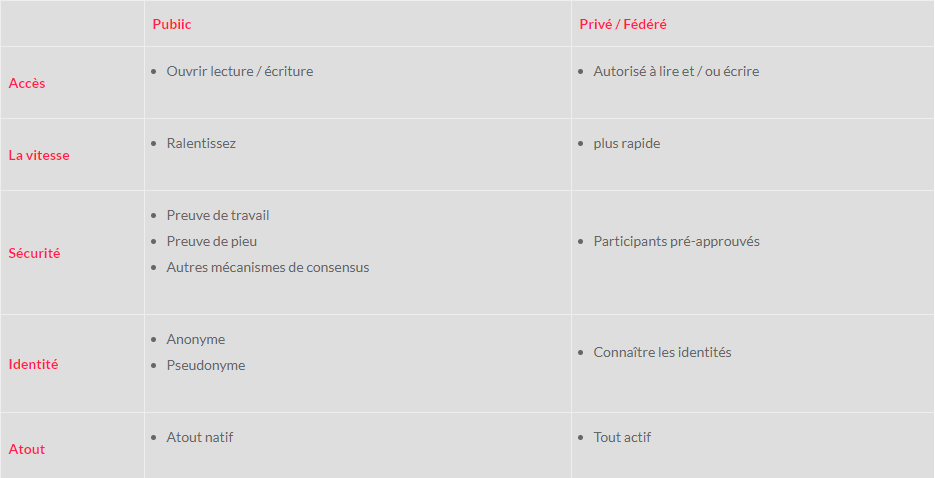
\includegraphics[width=1\textwidth]{shema_type_block.png}

    \textbf{\underline{Schéma de classification}} \\[1cm]
\end{center}

\hspace{1cm} Tous ces types de blockchains, publiques, privées et consortium, pourraient finir par cohabiter. Chacune est spécialisée sur des applications adéquates. Et comme le dit  \textbf{Luca Comparini}, un blockchain leader chez IBM France, je cite"La blockchain publique est idéale pour les marchés C2C et P2P, tandis que les blockchains privées et les consortiums sont davantage adaptés au B2B. Pour le B2C, cela dépendra des contraintes du secteur".  Ce qui pousse aux mineurs de prévoir des passerelles entre les différentes blockchains afin d'assurer leur une possibilité de communication entre les systèmes.\\


%%%%%%%%%%%%%% Système actuel %%%%%%%%%%%%%%
\newpage
\section{Système des transactions bancaires}

\hspace{1cm} Avant la mise en place des premières cartes de paiement, la plupart de la population gardait leurs fonds sur eux ou à leur domicile. Ce qui veut dire que ces sommes pouvaient être dérobées et quand ça arrivait ils n'étaient pas remboursés. Donc faire des achats n'était pas sans risque pour l'intégrité de l'acteur et de ses économies. De plus il fallait avoir la totalité de la somme du montant au moment d'un achat pour effectuer l'opération, ce qui rendait les transactions un peu compliquées. Il était aussi facile de faire des erreurs de calculs dès que la monnaie était échangée et les transactions bancaires n'était pas répertoriée directement.\\

\hspace{1cm} Pour faciliter les transactions bancaires, ils ont mis en place un système appelé la \textbf{monétique} qui regroupe l'ensemble des processus nécessaires à la création d'une carte, la lecture des informations associées et la gestion des transactions monétaires. Ces transactions monétaires ont toutes des processus différents et spécifique. Nous allons prendre comme exemple le processus d'une transaction par carte bancaire qui est très courant.Il met en jeux plusieurs acteurs tels que : 

\begin{itemize}
    \item Un \textbf{émetteur}, qui peut être la banque du client
    \item Un \textbf{porteur} de carte, c'est à dire le client
    \item Un \textbf{accepteur} du moyen de paiement qui est très souvent le commerçant
    \item Un \textbf{acquéreur} de données de transaction dont la banque émettrice
\end{itemize}

Ces principaux acteurs communiquent indirectement mais de façon coordonnée et sécurisée.En effet: 

\begin{itemize}
    \item il y a d'abord le client qui crée son compte dans une banque. La banque lui envoie une carte associée au compte et qui lui permettra de faire tous les achats par la suite.
    \item Dès lors le client est libre de faires ses transactions chez un commerçant. Parfois il peut y avoir des demandes d'autorisation afin de vérifier la solvabilité du compte ainsi que la validité de la carte.
    \item Après la transaction le commerçant obtient un TPE qui va lire la carte et transmettre les données de la transaction. Cette étape est appelée la \textbf{télécollecte}. 
    \item Une fois cette télécollecte effectuée, la banque du client et celle du commerçant communiquent entre elles afin d'effectuer ce qu'on appelle la \textbf{télécompensation} qui va permettre de débiter le compte du client et créditer celui du commerçant. \\[1cm]
\end{itemize}

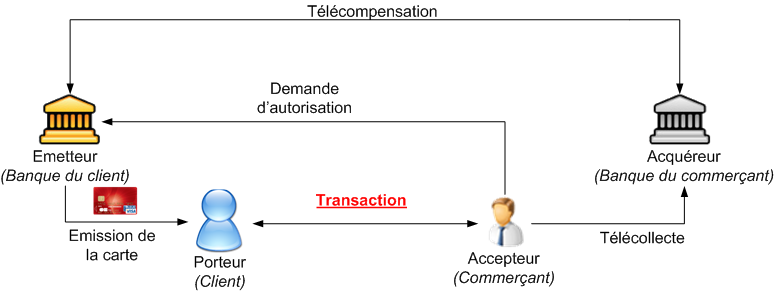
\includegraphics[width=1\textwidth]{process_transaction}
\begin{center}
   \textbf{\underline{Processus d'une transaction bancaire}} \\[1cm]
\end{center}

%%%%%%%%%%%%%% Carte bancaire %%%%%%%%%%%%%%
    \subsection{Les transactions par carte bancaire physique}
\hspace{1cm} La carte bancaire est le moyen de paiement le plus utilisé en France. Elle représente presque \textbf{50\%} des paiements en 2014 avec \textbf{9,49 milliards} de paiements effectués par cartes. Cette carte est d'une utilisation simple que ce soit pour un paiement ou pour un retrait et est acceptée presque par tous les commerçants.\\

\hspace{1cm} Cependant la carte nous impose un coût annuel assez élevé en fonction des banques ainsi que des frais sur certains retraits et paiements avec des assurances sur les achats effectués. De même il exige très souvent un montant minimum d'utilisation chez les commerçants. Ils ont mis en place des plafonnements de dépenses par mois ou par semaine en fonction des banques, ce qui est très embarrassant à cause du manque de flexibilité. Avec cette carte vous n'avez pas non plus la possibilité de faire des paiements entre particuliers. Et utiliser sa carte à l'étranger équivaut à payer des frais exorbitants.

%%%%%%%%%%%%%% E-commerce %%%%%%%%%%%%%%
    \subsection{Le monde du E-commerce}
\hspace{1cm} Le e-commerce est l'ensemble des transactions commerciales s'opérant à distance via des interfaces électroniques et digitales. Aujourd'hui c'est un secteur en pleine expansion. Les achats et ventes se passent le plus souvent par le biais du numérique au détriment des marchés physiques traditionnels. L'e-commerce prend de plus en plus d'ampleur. en effet, une étude de la Fevad montre un chiffre d'affaire qui s'élève à \textbf{72 milliards d'euro} en 2016 pour un total de plus de \textbf{200 000 sites marchands}. Nous avons environ \textbf{2000 euro par année} dépensé par un e-acheteur pour \textbf{28 transactions}. En 2016 l'e-commerce représentait \textbf{8\%} du commerce de détail.\\

\hspace{1cm} Par contre ces e-commerçants investissent beaucoup sur des plate-formes qui jouent le rôle d'intermédiaire entre eux et les acheteurs. Ce qui les pousse parfois à augmenter le prix de leurs marchandises pour en tirer bénéfice.\\ De même pour un paiement en ligne certains sites vous demanderont vos données personnelles, quelque chose dont vous ne connaissez où ça peut vous amener. Le manque de confiance dans les moyens de paiements sur les sites d'e-commerce et la peur de se faire arnaquer pose un vrai problème au grand public et porte préjudice aux e-commerçants. 


%%%%%%%%%%%%%% Transaction papier %%%%%%%%%%%%%%
    \subsection{Les transactions sur papier}
\hspace{1cm} Nous faisons différentes transactions basées principalement sur les documents telles que:

\begin{itemize}
    
    \item \textbf{Billet à ordre}: C'est un écrit par lequel le client s'engage à payer une certaine somme avec une échéance déterminée à son fournisseur.
    
    \item \textbf{Chèque}: C'est un écrit par lequel une personne donne l'ordre de payer une certaine somme, prélevable immédiatement sur les fonds portés au crédit de sont compte, à lui même ou à un tiers.
    
    \item \textbf{Lettre de change }: C'est un écrit par lequel un créancier d'origine donne à un débiteur l'ordre de payer avant l'échéance fixée, une certaine somme à une troisième personne appelée qui est le bénéficiaire.

\end{itemize}
    
\hspace{1cm} Ces moyens de transaction bancaires sont quotidiennement utilisés en France, particulièrement les chèques, grâce à leur gratuité d'acquisition. Avec une transaction par "papier", vous avez la possibilité de garder une trace du paiement.  De plus les paiements sont gratuits ainsi que leurs acquisitions.\\

\hspace{1cm} Mais il se trouve que certains commerçants n'acceptent pas les chèques à partir de certains montant, par mesure de sécurité et à cause  des nombreux chèque impayés. Effectivement vous n'avez aucune garantie que les chèques encaissés ne sont pas sans provisions. En plus de tout ça il y a beaucoup de fraudes sur les chèques aujourd'hui \\

%%%%%%%%%%%%%% Pret bancaire %%%%%%%%%%%%%%
    \subsection{Prêts bancaires}
    
\hspace{1cm} Faire un prêt consiste à remettre des fonds à un bénéficiaire, moyennant le plus souvent à un intérêt à verser au prêteur. Donc il y a un engagement de remboursement à respecter. Ces prêts sont profitables pour un financement à un projet et utiles pour tous ceux qui ont un besoin urgent. Mais le problèmes avec ces prêts c'est qu'ils vous proposent un taux d'intérêts élevés, augmentant ainsi le taux d'endettement. Ces prêts sont d'utilité mais à quel prix? Est ce qu'avec ce système ça vaut le coût ?


%%%%%%%%%%%%%% transfert d'argent %%%%%%%%%%%%%%
    \subsection{Les transferts d'argent}
    
Il existe plusieurs types de transferts  d'argent. Parmi eux nous pouvons en citer: 

\begin{enumerate}
    \item Virement bancaire: Ça consiste à envoyer ou recevoir de l'argent par le biais d'un compte bancaire. Vous avez la possibilité de faire des virements: 
    
    \begin{enumerate}
        \item ouverts dans la même banque, ce qu'on appelle \textbf{virement interne}
        \item ouverts dans deux banques différentes, appelé \textbf{virement externe}
        \item réalisés dans le même pays, appelé \textbf{virement domestique}
        \item réalisés entre deux pays de l'UE. Ce virement doit êre inférieur à \textbf{50 000 euros}
        \item réalisés hors UE, à l'étranger
        \item réalisés ponctuellement ou permanents 
    \end{enumerate}
Les virements bancaires sont des moyens de paiement à distance particulièrement utiles surtout s'il s'agit de grosses sommes ou de paiement de dépenses contraintes. \\

    \item Transfert d'argent à l'internationale: Nous pouvons en citer quelques uns : 
    
    \begin{enumerate}
        \item Mandat cash
        \item Western Union
        \item MoneyGram 
    \end{enumerate}
    
Les transferts d'argent par mandat cash ou western sont particulièrement destinés aux personnes ne détenant pas de compte bancaire. Ces transactions peuvent vous permettre d'envoyer de l'argent à une personne n'ayant pas de carte d'identité, mais avec maximum 400 euros.\\
    
\end{enumerate}

\hspace{1cm} Et pourtant, dès qu'on parle de transfert d'argent on se tourne vers les banques. On compte presque \textbf{600 milliards de dollars} envoyés dans le monde d’un pays à un autre par des particuliers par année. les banques utilisent des technologies dépassées et qui à cause du capitalisme rend ces transferts trop lents et trop chers. A ce jour  il est même possible de payer 1000 euros de frais pour juste envoyer 30000 euros et recevoir finalement l'argent 15 jours après. Donc ces transferts d’argent représentent beaucoup trop d’argent, partout, et dans plein de directions. Et les pays qui reçoivent le plus d’argent par leur population domiciliée à l’étranger sont l’Inde, le Mexique, les Philippine, la Chine ainsi que la France. Et inversement les pays qui font le plus d'argent sont les Etats Unis, l’Arabie Saoudite et la Suisse, parce que des gens y viennent de l’étranger, y gagnent un salaire assez confortable et le renvoient dans leur pays d’origine, et en plus les prix dans ces 3 pays sont trop élevés. \textbf{Voir annexe 2}\\

\hspace{1cm}Ces transferts sont très coûteux surtout à l'international.D'après les données de la Banque Mondiale en 2015,  presque \textbf{10\%} de commissions sont prélevés par les plateformes d’échange dans certaines régions. la diaspora africaine dépense ainsi \textbf{2 milliards d'euros} par an à cause des coûts d'envoi des transferts d'argent. Ces frais de transfert dont les coûts s'élèvent à \textbf{12\%}, soit le double de la moyenne mondiale. Il y a aussi les fluctuations de devise qui changent souvent les coûts.\\

%%%%%%%%%%%%%% Conclusion de ce chapitre %%%%%%%%%%%%%%
\hspace{1cm} Toutes ces transactions sont indispensables à notre quotidien. Mais il se trouve que nous avons des contraintes liées à leurs utilisations. Nous n'avons pas toujours ce que nous souhaitons et sommes parfois piégés par ce systèmes qui nous impose son processus ainsi que ses caprices.\\

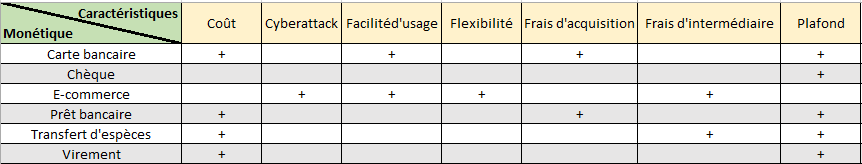
\includegraphics[width=1\textwidth]{tableau_recap}
\begin{center}
   \textbf{\underline{Récapitulatif du système actuel}} \\[1cm]
\end{center}


%%%%%%%%%%%%%% Blockchain %%%%%%%%%%%%%%
\newpage
\section{Blockchain dans les transactions}

\hspace{1cm} Nous vivons donc avec cette monétique qui nous permet d'effectuer des transactions bancaires, des transferts de fonds... Cependant ce système commence à semer les doutes dans l'esprit des utilisateurs. Il coûte de plus en cher et présente des failles de sécurité surtout avec la présence des cyberattacks sur le marché. Pour résoudre et faire face à ces problèmes, nous pouvons chercher d'autres méthodes pour assurer ces transactions. Et aucune autre technologie ne me vient en tête à part les blockchains. C'est vrai que c'est une nouvelle technologie, mais a déjà montré ses prouesses et semble avoir un avenir assuré. Je vais donc essayer de voir comment mettre en place les blockchains dans le monde monétaire, et plus précisément dans les transferts d'argent qui me semble être le domaine le plus impacté par notre système actuel. Et dans la mesure du possible, pourquoi ne pas aborder brièvement les autres transactions en interaction avec les blockchains? 

%%%%%%%%%%%%%% Transfert d'argent %%%%%%%%%%%%%%

    \subsection{La blockchain face aux transferts d'argent}

\hspace{1cm}Ces transferts qui prennent des jours pour arriver à destination avec des coûts très élevés peuvent prendre fin. Maie comment? Pourtant nous sommes à l'air de la blockchain. Cette technologie fait des miracles grâce à son système très sécurisé, rapide et efficace. Donc pourquoi ne pas passer par ce système pour résoudre notre problème et trouver une solution adéquate? Mais pour mieux expliquer cette solution je vais avant tout créer étape par étape une blockchain et essayer de l'exploiter et la mettre en oeuvre sur les transferts d'argent.

\subsection{Ma première blockchain en JAVA !!!!}

\hspace{1cm} Je vais partir sur la logique, vu ci-dessus, qu'une blockchain est, ni plus ni moins, qu'une liste de blocs. Par contre chaque block a sa propre signature numérique qu'on appellera \textbf{Hash} ici, contient le Hash du bloc précédent et dispose de certaines données comme des transactions. je vais définir dans chaque bloc non seulement le hachage du bloc précédent, mais aussi son propre hachage qui est en partie calculé à partir du hachage précédent.

\begin{lstlisting}

public class Block {

  public String hash;
  public String previousHash;
  
  //Les donnees sont juste un simple message stockes dans data.
  private String data; 
  
  //Pour l'horodatage, defini millisecondes.
  private long timeStamp;

  //Constructeur du bloc
  public Block(String data,String previousHash ) {
    this.data = data;
    this.previousHash = previousHash;
    this.timeStamp = new Date().getTime();
  }
}

\end{lstlisting}

Notre bloc de base , appelé souvent \textbf{genesis-block},est toujours codé en dur. Ainsi le bloc de base  contient un \textbf{String hash} qui va stocker notre signature numérique. La variable \textbf{previousHash}, quant à elle, contient le hachage du bloc précédent et enfin \textbf{String data} regroupe toutes nos données du bloc.\\

Générons maintenant notre signature numérique. Il existe plusieurs façons de le faire, comme vu précédemment, mais je vais choisir, parmi ces nombreux algorithmes cryptographiques, \textbf{SHA256} qui convient parfaitement pour notre cas.

\begin{lstlisting}

//Indispensable pour l'utilisation de l'algo SHA256
import java.security.MessageDigest;

public class StringUtil {

  //On applique Sha256 a notre chaine et qui va renvoyer le resultat.
  public static String algoSha256(String input){    
    try {
        MessageDigest digest = MessageDigest.getInstance("SHA-256");
      
   //On applique le sha256 a notre entree 
    byte[] hash = digest.digest(input.getBytes("UTF-8"));   
    
    //On stocke le hash comme hexadecimal
    StringBuffer stringBuffer = new StringBuffer(); 
    for (int i = 0; i < hash.length; i++) {
      String string = Integer.toStringBuffer(0xff & hash[i]);
    if(string.length() == 1) stringBuffer.append('0');
    stringBuffer.append(string);
    }
    return stringBuffer.toString();
  }
    catch(Exception e) {
    throw new RuntimeException(e);
  }
  } 
}
\end{lstlisting}

Ici, on prend une chaîne et lui applique l'algorithme SHA256 qui renvoie la signature générée sous forme de chaîne. Nous allons maintenant utiliser notre algoSha256 , dans une nouvelle méthode de la classe Block afin de calculer le hachage. Par contre nous devons calculer le hachage de toutes les parties du bloc que nous ne voulons pas altérer. Et pour cela nous inclurons le \textbf{previousHash}, le \textbf{data} et le \textbf{timeStamp}.

\begin{lstlisting}

public String calculateHash() {
  String calculatedhash = StringUtil.algoSha256( 
      previousHash +
      Long.toString(timeStamp) +
      data 
      );
  return calculatedhash;
}
\end{lstlisting}

On retourne initialiser cette méthode dans le constructeur. Ce qui nous donne 

\begin{lstlisting}

public Block(String data,String previousHash ) {
    this.data = data;
    this.previousHash = previousHash;
    this.timeStamp = new Date().getTime();
    this.hash = calculateHash(); 
  }
\end{lstlisting}

N'oublions pas qu'on avait dit qu'il existe un bloc de base qui n'a pas de précédent. Nous devons alors, si on suit la même logique, initialiser ce bloc à \textbf{0} dans notre classe principale \textbf{MyFirstBlockchain} qui permet de créer tous nos blocs.

\begin{lstlisting}

public class MyFirstBlockchain {

  public static void main(String[] args) {

    Block genesisBlock = new Block("block 1", "0");
    System.out.println("Hash pour block 1 : " + genesisBlock.hash);
		
    Block secondBlock = new Block("block 2",genesisBlock.hash);
    System.out.println("Hash pour block 2 : " + secondBlock.hash);
		
    Block thirdBlock = new Block("block 3",secondBlock.hash);
    System.out.println("Hash pour block 3 : " + thirdBlock.hash);
		
  }
}

\end{lstlisting}


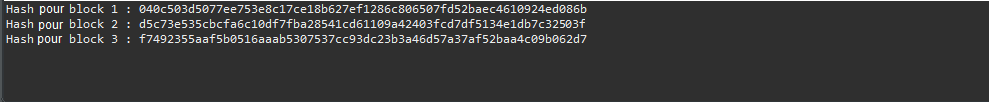
\includegraphics[width=1\textwidth]{result_b1.png}
\begin{center}
   \textbf{\underline{Premiers blocs créés}} \\[1cm]
\end{center}

Je viens de tester nos premiers blocs. Et bien vrai que chaque bloc a sa propre signature numérique basée sur ses informations et sur la signature du bloc précédent, nous n'avons pas encore une vraie chaîne de blocs. Et pour cela je vais stocker ces blocs dans une liste de blocs.

\begin{lstlisting}

import java.util.ArrayList;

//Pour visualiser sous Json
import com.google.gson.GsonBuilder;

public class MyFirstBlockchain {

  public static ArrayList<Block> blockchain = new ArrayList<Block>(); 

  public static void main(String[] args) {	
  
    //On ajoute nos blocs a la blockchain Liste 
    blockchain.add(new Block("block 1", "0"));		
    blockchain.add(new Block("block 2", 
                   blockchain.get(blockchain.size()-1).hash)); 
    blockchain.add(new Block("block 3", 
                   blockchain.get(blockchain.size()-1).hash));
	
    //Pour activer une jolie sortie
    String jsonBlockchain = new GsonBuilder().setPrettyPrinting().
                            create().toJson(blockchain);		
    System.out.println(jsonBlockchain);
  }

}
\end{lstlisting}

Nous venons de créer notre première blockchain. Maintenant passons à l'étape suivante.Il faut s'assurer de la sécurité de cette chaîne. Nous allons  vérifier l'intégrité de la blockchain. Nous allons créer une méthode booléenne dans notre classe principale afin de parcourir tous les blocs de la chaîne et comparer les hachages. Cette méthode nous permettra de vérifier si la variable de hachage est vraiment égale au hachage calculé et en même temps si le hachage du bloc précédent est égal à la variable previousHash qu'on avait calculer précédemment.

\begin{lstlisting}

public static Boolean isValidChain() {
  Block currentBlock; 
  Block previousBlock;
	
  //On boucle sur la blockchain pour verifier les hachages
  for(int i=1; i < blockchain.size(); i++) {
    currentBlock = blockchain.get(i);
    previousBlock = blockchain.get(i-1);
    
    //On compare le hachage enregistre et le hachage calcule
    if(!currentBlock.hash.equals(currentBlock.calculateHash()) ){
      System.out.println("Les hash actuels ne sont pas egaux");			
      return false;
    }
    //On compare le hash precedent et le hash precedent enregistre
    if(!previousBlock.hash.equals(currentBlock.previousHash) ) {
    System.out.println("Les hash precedents ne sont pas egaux");
    return false;
    }
  }
  return true;
}

\end{lstlisting}

Quiconque tente de modifier les blocs de la blockchain recevra un retour de cette méthode.\\

\hspace{1cm}Parlons un peu des Wallets. Un Wallet est une sorte de portefeuille, un logiciel dans lequel on stocke les monnaies cryptographique. mais en réalité la monnaie n'est pas vraiment stockée quelque part. Il existe une clé privée, ce qu'on appelle souvent \textbf{numéro secret} pour chaque adresse de monnaie enregistrée dans le Wallet de la personne qui détient le solde. Ainsi les Wallet facilitent l'envoi et la réception des monnaies et donnent à l'utilisateur la propriété du solde.Nous avons quatre principaux types de Wallet: \textbf{\textit{bureau}}, \textbf{\textit{mobile}}, \textbf{\textit{web}} et \textbf{\textit{matériel}}\\

\hspace{1cm} Essayons d'appliquer notre blockchain sur le Bitcoin en définissant le \textbf{Wallet Bitcoin}. En effet les nœuds du réseau, sur le bitcoin, partagent leurs chaînes de blocs et la plus longue chaîne valide est acceptée par le réseau. Mais qu'est ce qui peut empêcher à quelqu'un de changer des données dans un ancien bloc, puis de créer une nouvelle blockchain plus longue et de la présenter au réseau? Le \textbf{Proof of Work}. En effet le système de Proof of Work signifie qu'il faut beaucoup de temps et de puissance de calcul pour créer de nouveaux blocs. Par conséquent, l'attaquant aurait besoin de plus de puissance de calcul que le reste des pairs combinés.\\

\hspace{1cm} Pour mettre en place ce système nous avons besoin des \textbf{mineurs} pour le faire en essayant différentes valeurs de variables dans le bloc jusqu'à ce que leur hash commence par un certain nombre de 0. Nous allons reprendre notre classe \textbf{Block} et essayer de miner dessus.

\begin{lstlisting}

import java.util.Date;

public class Block {

  public String previousHash;
  public String hash;
  private long timeStamp;
  private String data;  
  private int nonce;
	
  //Constructeur du bloc
  public Block(String data,String previousHash ) {
    this.data = data;
    this.previousHash = previousHash;
    this.timeStamp = new Date().getTime();
    this.hash = calculateHash();
  }
	
  //Calcule du nouveau hash base sur le contenu des blocs
  public String calculateHash() {
    String calculatedhash = StringUtil.algoSha256( 
        previousHash +
        Long.toString(timeStamp) +
        Integer.toString(nonce) + 
        data 
            );
    return calculatedhash;
  }

  public void blockMine(int difficulty) {
  
     //On cree une chaine avec une difficulte * "0"
    String target = new String(new char[difficulty]).replace('\0', '0'); 
    while(!hash.substring( 0, difficulty).equals(target)) {
      nonce ++;
      hash = calculateHash();
    }
    System.out.println("Le bloc est mine : " + hash);
  }
}
\end{lstlisting}

\hspace{1cm} La nouvelle méthode \textbf{blockMine()} elle prend en compte une difficulté 0 que les mineurs doivent résoudre. Par contre une difficulté faible, comme par exemple  1 ou 2, peut être résolue presque instantanément sur la plupart des ordinateurs. 
Ici nous allons ajouter la difficulté en tant que variable statique à la classe. Mettons à jour notre classe principale afin de déclencher la méthode blockMine () pour chaque nouveau bloc.Nous allons donc appeler méthode \textbf{isValidChain ()} qui va faire la vérification sur les blocs.

\begin{lstlisting}

import java.util.ArrayList;
import com.google.gson.GsonBuilder;

public class MyFirstBlockchain {
	
  public static ArrayList<Block> blockchain = new ArrayList<Block>();
  
  //On fixe la difficulte a 5
  public static int difficulty = 5;

  public static void main(String[] args) {	
    
    //On va ajouter nos blocs a la blockchain	
    blockchain.add(new Block("block 1", "0"));
    System.out.println("Minage block 1");
    blockchain.get(0).blockMine(difficulty);
		
    blockchain.add(new Block("block 2", blockchain.
                             get(blockchain.size()-1).hash));
    System.out.println("Minage block 2");
    blockchain.get(1).blockMine(difficulty);
		
    blockchain.add(new Block("block 3", blockchain.
                             get(blockchain.size()-1).hash));
    System.out.println("Minage block 3 ");
    blockchain.get(2).blockMine(difficulty);	
		
    System.out.println("\n Cette blockchain est valide: " 
                       + isValidChain());
		
    String jsonBlockchain = new GsonBuilder().setPrettyPrinting().
                                            create().toJson(blockchain);
    System.out.println("\n Notre  chaine de bloc: ");
    System.out.println(jsonBlockchain);
  }

  //On fait la verification	sur les blocs
  public static Boolean isValidChain() {
    Block currentBlock; 
    Block previousBlock;
    String hashTarget = new String(new char[difficulty]).
                                   replace('\0', '0');
		
    //On boucle sur la blockchain pour verifier les hachages
    for(int i=1; i < blockchain.size(); i++) {
      currentBlock = blockchain.get(i);
      previousBlock = blockchain.get(i-1);
      
      //On compare le hachage enregistre et le hachage calcule:
      if(!currentBlock.hash.equals(currentBlock.calculateHash()) ){
        System.out.println("Les hash actuels ne sont pas egaux");			
        return false;
      }
      //On compare le hash precedent et le hash precedent enregistre
      if(!previousBlock.hash.equals(currentBlock.previousHash) ) {
        System.out.println("Les hash precedents ne sont pas egaux");
        return false;
      }
      //verifie si le hachage est resolu
      if(!currentBlock.hash.substring( 0, difficulty).equals(hashTarget)) {
        System.out.println("Ce bloc n'a pas ete mine ");
        return false;
      }
    }
    return true;
  }
}

\end{lstlisting}

\hspace{1cm} Si quelqu'un tentait de manipuler les données de notre système alors non seulement leur blockchain serait invalide mais ils ne seraient pas en mesure de créer une blockchain plus longue. Ainsi nous venons de mettre en place une blockchain : 
\begin{itemize}
    \item composée de blocs qui stockent des données. 
    \item qui possède une signature numérique permettant d'enchaîner nos blocs. 
    \item qui requiert une preuve de travail pour valider de chaque nouveau bloc.
    \item qui peut être vérifiée afin de voir si les données qu'elle contient sont valides et inchangées.
\end{itemize}

\hspace{1cm} Notre blockchain est vérifiable de base. Nous allons maintenant faire des transferts d'argent. Nous allons toujours partir sur le principe de Bitcoin et mettre en place notre pièce qu'on appellera \textbf{MyFirstCoins} en créant notre Wallet. \\
Maie faisons d'abord un tour du coté des crypto. En effet, en crypto-monnaies, les propriétés des pièces sont transférées sur la Blockchain comme étant des transactions. Les participants ont une adresse, en leur possession, vers laquelle les fonds sont envoyés. Dans leurs formulaires de base, les Wallets peuvent simplement stocker ces adresses, mais la plupart d'entre eux sont également des logiciels capables d'effectuer de nouvelles transactions sur la Blockchain.\\

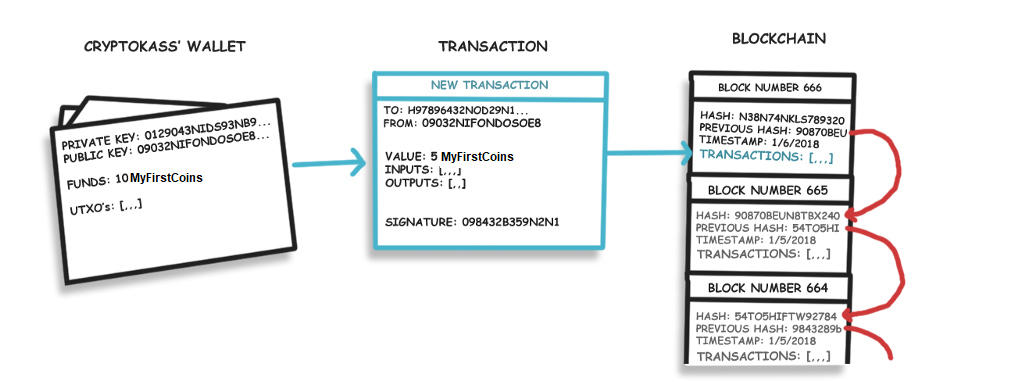
\includegraphics[width=1\textwidth]{wallet_trans.png}
\begin{center}
     \textbf{\underline{Transaction d'un wallet dans une la blockchain}} \\[1cm]
\end{center}


Créons maintenant notre Wallet pour y stocker nos clés privées notre clé publique.  
\hspace{1cm} La clé publique représentera l’adresse.C'est cette clé qui est partagée avec les autres pour recevoir les transferts. Quant à la clé privée, elle est utilisée pour signer les transactions, de telle sorte que personne ne puisse dépenser les coins autres que le propriétaire de la clé privée. Ainsi la clé privée est gardé secrètement alors que celle publique est envoyée avec la transaction. Et cela peut être utilisé pour vérifier que la signature est valide et que les données n'ont pas été falsifiées. Nous générons aussi nos clés publiques et privées dans un \textbf{KeyPair} .

\begin{lstlisting}

package MyFirstBlockchain;

/*Pour generer un KeyPair qui va creer et definir nos cles publique et 
privee */
import java.security.*;

public class Wallet {
	
  public PrivateKey privateKey;
  public PublicKey publicKey;
	
  public Wallet(){
    generateKeyPair();	
  }
		
  public void generateKeyPair() {
    try {
      KeyPairGenerator keyGenerator = KeyPairGenerator.
                                      getInstance("MASFE","FA");
      SecureRandom random = SecureRandom.getInstance("SHA1PRNG");
      ECGenParameterSpec ecgSpec = new ECGenParameterSpec("prime0105");
      
      // On initialise le generateur de cle et on genere un KeyPair
      keyGenerator.initialize(ecgSpec, random);
      KeyPair keyPair = keyGenerator.generateKeyPair();
      
      // On definit les cles publiques et privees du keyPair
      privateKey = keyPair.getPrivate();
      publicKey = keyPair.getPublic();
      
    }catch(Exception e) {
      throw new RuntimeException(e);
	}
  }
}
\end{lstlisting}

\hspace{1cm} Maintenant que nous avons mis en place les bases pour notre Wallet, regardons les transactions. Chaque transaction a un certain nombre de données comme :

\begin{itemize}
    \item une clé publique (adresse) de l'expéditeur des fonds.
    \item une clé publique (adresse) du destinataire des fonds.
    \item la valeur / montant des fonds à transférer.
    \item des entrées, qui sont des références à des transactions précédentes qui prouvent que l'expéditeur a des fonds à envoyer.
    \item des sorties indiquant le montant des adresses pertinentes reçues dans la transaction.
    \item une signature cryptographique, qui prouve que le propriétaire de l'adresse est celle qui envoie cette transaction et que les données n'ont pas été modifiées.
\end{itemize}
Mais quel est le but réel de ces signatures et comment fonctionnent-elles? En fait,
les signatures exécutent deux tâches très importantes sur notre blockchain: premièrement, elles permettent uniquement au propriétaire de dépenser ses pièces ; deuxièmement, elles empêchent les autres de manipuler leur transaction avant l’exploitation d’un nouveau bloc (par exemple au point d’entrée).

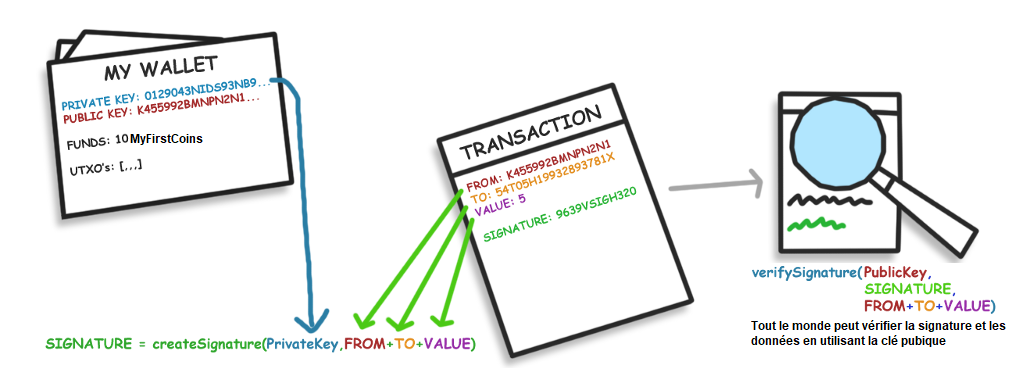
\includegraphics[width=1\textwidth]{wallet_trans_key.png}   
\begin{center}
   \textbf{\underline{Transaction \& Signature}} \\[1cm]
\end{center}

Créons ensuite notre classe de transaction. Cette classe contiendra les méthodes pour générer / vérifier la signature et vérifier la transaction.

\begin{lstlisting}

import java.security.*;
import java.util.ArrayList;

public class Transaction {

  //Le hash de la transaction	
  public String idTransaction; 
  
  //Adresse de l'expediteur
  public PublicKey sender; 
  
  //Adresse du destinaire
  public PublicKey reciepient; 
  public float value;
  
  //Pour empecher aux autres de depenser des fonds dans notre Wallet.
  public byte[] signature; 
	
  public ArrayList<TransactionInput> inputs = 
                                    new ArrayList<TransactionInput>();
  public ArrayList<TransactionOutput> outputs = 
                                    new ArrayList<TransactionOutput>();
  //Pour compter approximatif le nombre de transactions generees.
  private static int sequence = 0;
	
  // Constructeur: 
  public Transaction(PublicKey from, PublicKey to, float value, 
                    ArrayList<TransactionInput> inputs) {
    this.sender = from;
    this.reciepient = to;
    this.value = value;
    this.inputs = inputs;
  }
    
  // On calcule le hash de la transaction
  private String calulateHash() {
  
    /*On incremente la sequence pour eviter 2 transactions identiques 
    ayant le meme hachage*/
    sequence++;
    return StringUtil.algoSha256(
                        StringUtil.getStringFromKey(sender) +
                        StringUtil.getStringFromKey(reciepient) +
                        Float.toString(value) + sequence
                    );
  }
}

\end{lstlisting}

Nous pouvons voir (à partir du bloc de code précédent) que notre signature sera un paquet d’octets, alors créons une méthode pour les générer. La première chose dont nous aurons besoin est quelques fonctions d'aide dans la classe StringUtil  :

\hspace{1cm} Nous savons maintenant que notre signature sera un paquet d’octets, on va créer une petite  méthode pour les générer\\

\begin{lstlisting}

  //On applique la signature MASFE et renvoie le resultat
  public static byte[] algoMASFESig(PrivateKey privateKey, String input) {
    Signature dsa;
    byte[] output = new byte[0];
    try {
      dsa = Signature.getInstance("ECDSA", "BC");
      dsa.initSign(privateKey);
      byte[] strByte = input.getBytes();
      dsa.update(strByte);
      byte[] realSig = dsa.sign();
      output = realSig;
		
    }catch (Exception e) {
        throw new RuntimeException(e);
    }
    return output;
 }
	
  //on verifie la  signature de chaine
  public static boolean verifyMASFESig(PublicKey publicKey, String data, 
                                        byte[] signature) {
    try {
      Signature masfeVerify = Signature.getInstance("MASFE", "FA");
      masfeVerify.initVerify(publicKey);
      masfeVerify.update(data.getBytes());
      return masfeVerify.verify(signature);
    
    }catch(Exception e) {
      throw new RuntimeException(e);
    }
  }

  public static String getStringFromKey(Key key) {
    return Base64.getEncoder().encodeToString(key.getEncoded());
  }
\end{lstlisting}

\hspace{1cm}Ici \textbf{algoMASFESig} prend en compte le signe, la clé privée et la chaîne de caractères de l'expéditeur  et renvoie un tableau d'octets. \\ 
verifyMASFESig prend les données de signature, de clé publique et de chaîne et renvoie \textbf{vrai} ou \textbf{faux} si la signature est valide. getStringFromKey quant à elle renvoie une chaîne codée à partir de n'importe quelle clé.\\
Utilisons maintenant ces méthodes de signature dans notre classe Transaction 

\begin{lstlisting}

//On signe toutes les donnees que nous ne souhaitons pas etre alterees
public void generateSignature(PrivateKey privateKey) {
  String data = StringUtil.getStringFromKey(sender) +
  StringUtil.getStringFromKey(reciepient) + Float.toString(value)	;
  signature = StringUtil.algoMASFESig(privateKey,data);		
}

//On verifie que les donnees que nous avons signees n ont pas ete falsifiees
public boolean verifySignature() {
  String data = StringUtil.getStringFromKey(sender) +
  StringUtil.getStringFromKey(reciepient) + Float.toString(value);
  
  return StringUtil.verifyECDSASig(sender, data, signature);
}

\end{lstlisting}

\hspace{1cm} Et c'est à ce moment là que les mineurs vérifient les signatures car une nouvelle transaction est ajoutée à un bloc. Mais on peut également vérifier les signatures, lorsqu'on vérifie la validité de la blockchain.\\
Nous allons attaquer la dernière partie de notre code. Nous allons tester tout ceci sur un transfert. Reprenons notre classe principale

\begin{lstlisting}

import java.security.Security;
import java.util.ArrayList;
import java.util.Base64;
import com.google.gson.GsonBuilder;

public class MyFirstBlockchain {
	
  public static ArrayList<Block> blockchain = new ArrayList<Block>();
  public static int difficulty = 5;
  public static Wallet walletA;
  public static Wallet walletB;

  public static void main(String[] args) {
  
    //On configure le fournisseur de securite
    Security.addProvider(new org.bouncycastle.jce.provider.
                         BouncyCastleProvider()); 
    
    //On cree les nouveaux wallets
    walletA = new Wallet();
    walletB = new Wallet();
    
    //On teste les cles privees et publique
    System.out.println("Private and public keys:");
    System.out.println(StringUtil.getStringFromKey(walletA.privateKey));
    
    //On cree une transaction de WalletA a WalletB
    Transaction transaction = new Transaction(walletA.publicKey, 
                                walletB.publicKey, 5, null);
    transaction.generateSignature(walletA.privateKey);
    
    //On verifie signature et la cle publique
    System.out.println("Est-ce que la signature est verifiee ");
    System.out.println(transaction.verifySignature());
 }
}

\end{lstlisting}

\hspace{1cm} Nous venons de créer les Wallet A et B et imprimer nos clés  privées et publiques de Wallet A. Nous avons généré la transaction et la signature grâce à la clé privée du Wallet A. Nous pouvons maintenant créer et vérifier les entrées et les sorties pour enfin stocker la transaction dans la blockchain. Prenons exemple du Bitcoin, pour en posséder un, vous devez en recevoir un. On n'ajoute pas vraiment un bitcoin à vous et moins un bitcoin de l'expéditeur, l'expéditeur mentionne qu'il avait déjà reçu un bitcoin, puis une sortie de transaction a été créée indiquant qu'1 Bitcoin a été envoyé à votre adresse. Le solde de votre Wallet est la somme de toutes les sorties de transaction non dépensées qui vous sont adressées. De ce fait nous allons suivre la \textbf{convention bitcoins} et appellerons les sorties de transaction non dépensées: les \textbf{UTXO} . Pour cela on va retourner sur les transactions et créer nos classes en entrée \textbf{TransactionInput} et en sortie \textbf{TransactionOutputs}. 

\begin{lstlisting}

public class TransactionInput {

  //Reference a TransactionOutputs -> transactionId
  public String transactionOutputId; 
  
  //Elle contient la sortie de transaction non depensee
  public TransactionOutput UTXO;
	
  public TransactionInput(String transactionOutputId) {
    this.transactionOutputId = transactionOutputId;
  }
}
\end{lstlisting}

\hspace{1cm} Notre classe TransactionInput est utilisée pour référencer la classe TransactionOutputs dont les fonds n'ont pas encore été dépensés. La transactionOutputId, utilisée plutôt pour trouver le TransactionOutput approprié , va permettre aux mineurs de vérifier la propriété.

\begin{lstlisting}

public class TransactionOutput {

  public String id;
  
  //Le nouveau detenteur de ces pieces.
  public PublicKey reciepient; 
  
  //L'id de la transaction dans laquelle cette sortie a ete creee
  public String parentTransactionId; 
  
  //La quantite de pieces qu'on possede
  public float value; 
  
	
  //Constructeur
  public TransactionOutput(PublicKey reciepient, float value, 
                            String parentTransactionId) {
    this.reciepient = reciepient;
    this.value = value;
    this.parentTransactionId = parentTransactionId;
    this.id = StringUtil.algoSha256(StringUtil.
                                getStringFromKey(reciepient)+Float.
                                toString(value)+parentTransactionId);
  }
	
  //On verifie si lapiece vous appartient
  public boolean isMine(PublicKey publicKey) {
    return (publicKey == reciepient);
  }
}
\end{lstlisting}

\hspace{1cm} Les sorties de transaction indiquent le montant final envoyé à chaque étape de la transaction. Ces dernières agissent comme une preuve que vous avez des pièces à envoyer quand elles sont référencées comme étant des entrées dans de nouvelles transactions. Les blocs de la chaîne peuvent aussi recevoir de nombreuses transactions et la blockchain peut être très longue, ce qui peut prendre des années pour traiter une nouvelle transaction puisque nous devons rechercher et vérifier toutes les entrées. Mais pour éviter ce temps d'attente nous conservons une sorte de collection supplémentaire de toutes les transactions non dépensées pouvant être utilisées. Ajoutons donc cette collection de tous les UTXO.

\begin{lstlisting}

public class MyFirstBlockchain {
	
  public static ArrayList<Block> blockchain = new ArrayList<Block>();
  public static HashMap<String,TransactionOutputs> UTXOs = new
	
  /*liste de toutes les transactions non depensees.
  Cette liste nous permet d'utiliser une cle pour trouver une valeur*/
  HashMap<String,TransactionOutputs>(); 
  
  public static int difficulty = 5;
  public static Wallet walletA;
  public static Wallet walletB;
	
  /*...........................*/
}	
\end{lstlisting}

\hspace{1cm}Rassemblons tous ces bouts de code pour afin traiter la transaction avec notre nouvelle méthode booléenne \textbf{treatementTransaction} dans notre classe de transaction. Ce qui nous donne:

\begin{lstlisting}

//On envoi true si une nouvelle transaction peut etre creee
public boolean treatementTransaction() {
		
  if(verifySignature() == false) {
    System.out.println("La signature n'a pas pu etre verifiee ");
    return false;
  }
				
  //on rassemble les entrees de transaction
  for(TransactionInput i : inputs) {
    i.UTXO = MyFirstBlockchain.UTXOs.get(i.transactionOutputId);
  }

  //On verifie si la transaction est valide ou pas
  if(getInputsValue() < MyFirstBlockchain.minimumTransaction) {
    System.out.println("#Transaction Inputs to small: " + getInputsValue());
    return false;
  }
		
  /*On verifie si la transaction est valide
  et recupere la valeur des entrees puis le reste de la modification */
  float modifValue = getInputsValue() - value; 
  transactionId = calulateHash();
  
  // On envoie la valeur au destinataire
  outputs.add(new TransactionOutput( this.reciepient, value,transactionId)); 
  
  // On renvoie le "changement" a l'expediteur
  outputs.add(new TransactionOutput( this.sender, modifValue,transactionId)); 
				
  // On ajoute des sorties a la liste non depensee
  for(TransactionOutput o : outputs) {
    MyFirstBlockchain.UTXOs.put(o.id , o);
  }
		
  //On supprime les entrees de transaction des listes UTXO comme depensee
  for(TransactionInput i : inputs) {
    if(i.UTXO == null)
      continue;
    MyFirstBlockchain.UTXOs.remove(i.UTXO.id);
  }
		
  return true;
}
	
/On renvoie la somme des valeurs des entrees
public float getInputsValue() {
  float total = 0;
  for(TransactionInput i : inputs) {
    if(i.UTXO == null) continue; //if Transaction can't be found skip it 
      total += i.UTXO.value;
  }
  return total;
}

//On retourne la somme des sorties
public float getOutputsValue() {
  float total = 0;
  for(TransactionOutput o : outputs) {
    total += o.value;
  }
  return total;
}
	
\end{lstlisting}

\hspace{1cm}Grâce à cette méthode, nous effectuons des vérifications afin de nous assurer que la transaction est valide, puis collectons les entrées et générons les sorties. Ensuite, vers la fin, nous rejetons les entrées de notre liste UTXO, ce qui signifie qu'une sortie de transaction ne peut être utilisée qu'une seule fois en entrée. D'où la valeur totale des entrées doit donc être utilisée pour que l'expéditeur l'expéditeur envoie le changement de retour à sur lui même.\\

\hspace{1cm} Maintenant que notre système de transaction fonctionne, nous allons l'implémenter dans notre blockchain. Nous allons remplir les blocs par une liste de transactions. Par contre, il peut y avoir des milliers de transactions dans un seul bloc, trop nombreuses pour être incluses dans notre calcul de hachage. Mais dans ces cas là on utilise la racine de \textbf{merkle} des transactions. Ajoutons cette méthode pour générer d'abord le \textbf{merkleroot}.

\begin{lstlisting}

/*On remplie le tableau de transactions et renvoie 
une racine de type merkle*/
public static String getMerkleRoot(ArrayList<Transaction> transactions){

  int count = transactions.size();
  ArrayList<String> previousTreeLayer = new ArrayList<String>();
  for(Transaction transaction : transactions) {
    previousTreeLayer.add(transaction.transactionId);
  }
  
  ArrayList<String> treeLayer = previousTreeLayer;
  while(count > 1) {
    treeLayer = new ArrayList<String>();
    for(int i=1; i < previousTreeLayer.size(); i++) {
      treeLayer.add(algoSha256(previousTreeLayer.get(i-1) + 
                    previousTreeLayer.get(i)));
    }
    count = treeLayer.size();
    previousTreeLayer = treeLayer;
  }
  
  String merkleRoot = (treeLayer.size() == 1) ? treeLayer.get(0) : "";
  return merkleRoot;
}

\end{lstlisting}
Appliquons cette merkleroot dnas notre implémentation

\begin{lstlisting}

import java.util.ArrayList;
import java.util.Date;

public class Block {
	
  public String merkleRoot;
  public String hash;
  public String previousHash;  
  public ArrayList<Transaction> transactions = 
                                        new ArrayList<Transaction>(); 
  public long timeStamp;
  public int nonce;
	
  //Constructeur.  
  public Block(String previousHash ) {
    this.previousHash = previousHash;
    this.timeStamp = new Date().getTime();
		
    this.hash = calculateHash();
  }
	
  //On calcule un nouveau hash base sur le contenu des blocs
  public String calculateHash() {
    String calculatedhash = StringUtil.algoSha256( 
                            previousHash +
                            Long.toString(timeStamp) +
                            Integer.toString(nonce) + 
                            merkleRoot
                        );
    return calculatedhash;
  }
	
  //On augmente la valeur de nonce jusqu'a ce que la cible de hachage soit atteinte.
  public void mineBlock(int difficulty) {
    merkleRoot = StringUtil.getMerkleRoot(transactions);
    
    //On cree une chaine avec difficulte =  "0"
	String target = StringUtil.getDificultyString(difficulty); 
    while(!hash.substring( 0, difficulty).equals(target)) {
      nonce ++;
      hash = calculateHash();
    }
    System.out.println("Block Mined!!! : " + hash);
  }
	
    //On ajoute des transactions a ce bloc
    public boolean addTransaction(Transaction transaction) {
    
      /*On traite la transaction et verifie si elle est valide
      si le block coincide avec genesis block on ignore */
      if(transaction == null) 
        return false;	
      if((previousHash != "0")) {
        if((transaction.treatementTransaction() != true)) {
          System.out.println("Transaction failed. Delete.");
          return false;
        }
      }
      transactions.add(transaction);
      System.out.println("Transaction Successfully added to Block");
      return true;
    }
}
\end{lstlisting}

\hspace{1cm}Nous avons tous les éléments pour tester notre blockchain avec l'envoi des pièces Wallet à un autre. Nous allons partir de notre \textbf{block genesis} en le codant tout simplement. Nous allons aussi mettre à jour notre classe mère avec tout ce dont elle a besoin à savoir un contrôle de validité de la chaîne qui prend en compte les transactions et quelques transactions de test pour montrer que tout fonctionne.

\begin{lstlisting}

public class MyFirstBlockchain {
	
  public static int difficulty = 3;
  public static float minimumTransaction = 0.1f;
  public static Wallet walletA;
  public static Wallet walletB;
  public static Transaction genesisTransaction;
  
  public static ArrayList<Block> blockchain = new ArrayList<Block>(); 
  public static HashMap<String,TransactionOutput> UTXOs = new HashMap<String,TransactionOutput>();

  public static void main(String[] args) {	
    //On ajoute nos blocs a la blockchain ArrayList
    Security.addProvider(new org.bouncycastle.jce.provider.
                         BouncyCastleProvider());
		
    //On cree les wallets:
    walletA = new Wallet();
    walletB = new Wallet();		
    Wallet coinbase = new Wallet();
		
    //cree une transaction de genese, qui envoie 100 coins a walletA
    genesisTransaction = new Transaction(coinbase.publicKey, 
                         walletA.publicKey, 100f, null);
                         
    //On signe manuellement la transaction de genese
    genesisTransaction.generateSignature(coinbase.privateKey);
    
    //On definit manuellement l'identifiant de la transaction
    genesisTransaction.transactionId = "0"; 
    
    //On ajoute manuellement la sortie des transactions
    genesisTransaction.outputs.add(
        new TransactionOutput(genesisTransaction.reciepient, 
            genesisTransaction.value, genesisTransaction.transactionId)); 
    
    // On stocke notre premiere transaction dans la liste des UTXO
    UTXOs.put(genesisTransaction.outputs.get(0).id, genesisTransaction.outputs.get(0)); 
		
    System.out.println("Creating and Mining Genesis block... ");
    Block genesis = new Block("0");
    genesis.addTransaction(genesisTransaction);
    addBlock(genesis);
		
    //On teste tout
    Block block1 = new Block(genesis.hash);
    System.out.println("\n WalletA's balance is:"+ walletA.getBalance());
    System.out.println("\n WalletA is Attempting to send funds (40) 
                        to WalletB...");
    block1.addTransaction(walletA.sendFunds(walletB.publicKey, 40f));
    addBlock(block1);
    System.out.println("\n WalletA's balance is: " + walletA.getBalance());
    System.out.println("WalletB's balance is: " + walletB.getBalance());
		
    Block block2 = new Block(block1.hash);
    System.out.println("\n WalletA Attempting to send more funds (1000)
                        than it has...");
    block2.addTransaction(walletA.sendFunds(walletB.publicKey, 1000f));
    addBlock(block2);
    System.out.println("\n WalletA's balance is:"+ walletA.getBalance());
    System.out.println("WalletB's balance is:"+ walletB.getBalance());
		
    Block block3 = new Block(block2.hash);
    System.out.println("\n WalletB is Attempting to send funds (20)
                        to WalletA...");
    block3.addTransaction(walletB.sendFunds( walletA.publicKey, 20));
    System.out.println("\nWalletA's balance is:"+ walletA.getBalance());
    System.out.println("WalletB's balance is:"+ walletB.getBalance());
		
    isChainValid();
		
  }
	
  public static Boolean isChainValid() {
    Block currentBlock; 
    Block previousBlock;
    String hashTarget = new String(new char[difficulty]).
                        replace('\0','0');
    
    /*On garde une liste de travail temporaire des transactions 
    non depensees a un etat de block donne */
    HashMap<String,TransactionOutput> tempUTXOs = 
                                    new HashMap<String,TransactionOutput>();
    tempUTXOs.put(genesisTransaction.outputs.get(0).id, 
                    genesisTransaction.outputs.get(0));
		
    //On boucle sur la blockchain pour verifier les hachages
    for(int i=1; i < blockchain.size(); i++) {
      currentBlock = blockchain.get(i);
      previousBlock = blockchain.get(i-1);
      
      //On compare le hachage enregistre et le hachage calcule
      if(!currentBlock.hash.equals(currentBlock.calculateHash()) ){
        System.out.println("Current Hashes not equal");
        return false;
      }
      //On compare le hash precedent et le hash precedent enregistre
      if(!previousBlock.hash.equals(currentBlock.previousHash) ) {
        System.out.println("Previous Hashes not equal");
        return false;
      }
        
      //On verifie si le hachage est resolu
      if(!currentBlock.hash.substring(0,difficulty).
            equals(hashTarget)){
        System.out.println(" This block hasn't been mined");
        return false;
      }
			
      //On boucle sur les transactions blockchains
      TransactionOutput tempOutput;
      for(int t=0; t <currentBlock.transactions.size(); t++) {
        Transaction currentTransaction=currentBlock.transactions.get(t);
				
        if(!currentTransaction.verifySignature()) {
          System.out.println("Sign on Transaction("+ t +")is Invalid");
          return false; 
        }
        
        if(currentTransaction.getInputsValue() != currentTransaction.
                            getOutputsValue()) {
          System.out.println("Inputs are note equal to outputs 
                                on Transaction(" + t + ")");
          return false; 
        }
				
        for(TransactionInput input: currentTransaction.inputs) {	
          tempOutput = tempUTXOs.get(input.transactionOutputId);
					
          if(tempOutput == null) {
            System.out.println("#Referenced input on Transaction("+ t +") 
                                is Missing");
            return false;
          }
					
          if(input.UTXO.value != tempOutput.value) {
            System.out.println("#Referenced input Transaction("+ t +") 
                                value is Invalid");
            return false;
          }
					
          tempUTXOs.remove(input.transactionOutputId);
        }
				
        for(TransactionOutput output: currentTransaction.outputs) {
          tempUTXOs.put(output.id, output);
        }
				
        if( currentTransaction.outputs.get(0).reciepient != 
                        currentTransaction.reciepient) {
          System.out.println("#Transaction(" + t + ") 
                        output reciepient is not who it should be");
          return false;
        }

        if( currentTransaction.outputs.get(1).reciepient != 
                currentTransaction.sender) {
          System.out.println("#Transaction(" + t + ") 
                                output 'change' is not sender.");
          return false;
        }
				
      }
			
    }
    System.out.println("Blockchain is valid");
    return true;
  }
	
  public static void addBlock(Block newBlock) {
    newBlock.mineBlock(difficulty);
    blockchain.add(newBlock);
  }
}

\end{lstlisting}

Nous pouvons à présenter avoir un résultat concret de notre blockchain avec les transactions.

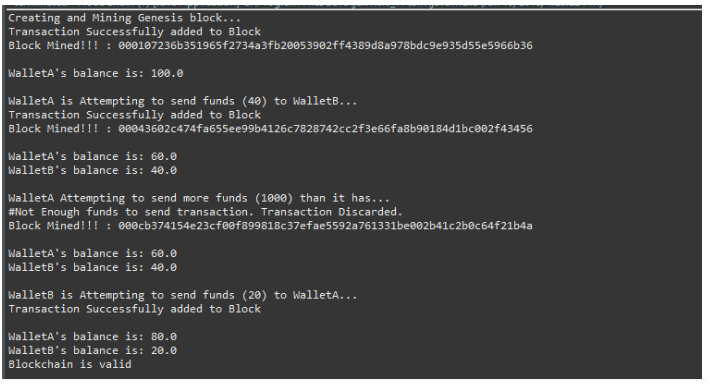
\includegraphics[width=1\textwidth]{result_final.png}
\begin{center}
   \textbf{\underline{Les transactions dans notre blockchain }} \\[1cm]
\end{center}

\hspace{1cm} Nous avons une blockchain opérationnelle, prête à être utilise et qui nous donne la possibilité de faire des transferts en toute sécurité.

\hspace{1cm} Nous avons montré un peu avant que les partenaires, les intermédiaires nous coûtent chers pour faire les transferts d'argent. De plus faire un virement prend des jours pour arriver à destinations. Utiliser la technologie de la blockchain rend les transferts plus rapides et moins chers. Pour cela on peut utiliser nos algorithmes. Nous venons de voir que peu importe l'endroit ou on est, si on veut transférer des fonds on passe par les Wallets et envoyer la somme qu'on veut donc les transferts entres l’Europe et le Mexique est bien possible.\\

\hspace{1cm} \textbf{Comment faire ces transferts d'argent en utilisant notre blockchain?}\\
Pour faire tourner notre blockchain un seul développeur ne nous suffira pas. il nous en faut plusieurs , les mineurs, pour faire tourner les algos. Et supposons qu'ici nous avons 10 mineurs et 2 particuliers qui détiennent un Wallet chacun, walletA et walletB. Maintenant ParticulierA souhaite envoyer 100 euros à ParticulierB. Sa requête va arriver en tant que message \textbf{"Je souhaite envoyer 100 euross à ParticulierB} à nos 10 mineurs. Le mineurs vérifient que ParticulierA possède suffisamment d’argent pour pouvoir effectuer ce transfert. Ils vont s'assurer que le  walletA détient bien les fonds. Si tel est  le cas, ils font appel aux classe \textbf{TransactionInput} et \textbf{TransactionOutputs} pour effectuer la transaction. Sachant qu'ils ont bien respecté au préalable la procédure de la sécurisation, des clés privée et publique.\\

\hspace{1cm} Ainsi la blockchain nous offre 2 possibilités de transférer de l'argent:
\begin{itemize} 
    \item Soit ParticulierA qui habite en Europe veut envoyer 1000 euros à ParticulierB qui vit aux USA. ParticulierA va acheter X bitcoins en France (l’équivalent de 1000 euros) sur un site comme Coinbase. Il envoie les bitcoins à ParticulierB aux USA qui aura préalablement ouvert un compte sur Coinbase aux USA. Et lui de son compte crypto aux USA, il peut vendre les bitcoins et recevoir des dollars sur son compte bancaire en échange. Donc les seuls frais possibles ici sera pour ouvrir un compte Coinbase.
    
    \item Soit ParticulierA crée, comme on a fait un peu plus en haut, un algorithme qui une fois les fonds transformés en BTC, envoie à la seconde près les BTC aux USA et les convertit instantanément en dollar de telle sorte que les quelques minutes du transfert limitent la volatilité (qui doit être tenu en compte) à un niveau inférieur à 0.1\% en moyenne, ce qui permet de faire France-> USA pour moins de 1\% de frais, ce qui représente 3 à 10 fois moins que le tarif pratiqué par les banques.
\end{itemize}


%%%%%%%%%%%%%% Carte bancaire %%%%%%%%%%%%%%

    \subsection{Autres transactions bancaires}
    
    \begin{enumerate}
    
        \item \textbf{Carte bancaire}
   

\hspace{1cm} Le système de la blockchain pourrait aussi faire disparaître les contraintes liées aux cartes bancaires et nous offrir ainsi une meilleure gestion de nos transactions. Et quoi de plus beau que de pouvoir dépenser ses \textit{coins} dans la boulangerie en bas de chez soi? Pourtant c'est bien possible en mettant en place des cartes bancaires en crypto-monnaie. Cette carte est reliée à votre wallet, qui stocke "votre richesse". Et afin d'effectuer des transactions de manière décentralisée, le wallet doit en sorte être "multi-cryptos. C'est à dire donner accès à plusieurs devises virtuelles dans différentes chaînes de blocs, afin de ne pas imposer aux utilisateurs une unique monnaie. \\

\hspace{1cm} Cette carte permettra aussi de dépenser ses cryptomonnaies chez le commerçant qui, à priori, n'a pas à y voir un quelconque inconvénient. En effet pour lui c'est comme une carte bancaire normale puisqu'il recevra son argent en euro. Tout simplement parce que la conversion crypto en euro est instantanée. Comment ça marche? Lorsque vous effectuez un paiement chez le commerçant, une vente instantanée du même montant en crypto est donc initiée. La carte est ensuite chargée du montant en euro, sans laisser de trace et sans que le commerçant même sans aperçoive.\\

\hspace{1cm} La carte sera transparente aussi pour tout ce qui est frais bancaire, donc pratiquement pas de frais du tout, même si une transaction en bitcoin coûte de plus en plus chère. Il faut afficher continuellement les cours auxquels les cryptomonnaies seront vendus en se basant sur plusieurs échanges afin de proposer le meilleur taux. Mais à vrai dire, un paiement sans frais n'existe pas, donc qui doit payer les frais? Sur ce point il n y aura pas de changement car ce sera le marchand qui paie comme dans les transactions bancaires actuelles.\\


%%%%%%%%%%%%%% E-commerce %%%%%%%%%%%%%%

     \item \textbf{Le E-commerce}

\hspace{1cm} Cette blockchain serait un grand atout pour ces e-commerçants. En effet la mise en place de cette technologie dans ce secteur supprimerait tous les intermédiaires entre vendeurs et acheteurs. Les e-commerçants pourront proposer des transactions se passant d'intermédiaires, donc ne plus verser de commissions aux plate-formes, aux organismes bancaires. Prenons un exemple sur Shopify et Paypal, qui sont des sociétés de paiement en ligne très populaires de grandes plate-formes de commerce. Elles prennent une commission de 1,5\% à 6\%. Cette redevance est transmise au client, ce qui rend les achats en ligne beaucoup plus chers.\\

\hspace{1cm} D'après \textbf{Thomas France}, co-fondateur de la Maison du Bitcoin à Paris, ce système pourrait faire économiser 3\% à 4\% des chiffres d'affaires des e-commerçants qui réalisent beaucoup d'opérations depuis de l'étranger. Effectivement, les transactions internationales sont souvent réalisées par l'intermédiaire des plate-formes tierces, les obligeant à débourser beaucoup de frais. Alors que les paiements en bitcoins ne génèrent aucun frais de transactions pour le vendeur. Ceci est un grand avantage pour les e-commerçants en quête de rentabilité absolue.\\

\hspace{1cm} L'inexistence des frais de transaction est assurée grâce au protocole de la blockchain dont le code source a la caractéristique d'être un open source. De même avec son fonctionnement sur le réseau de pair à pair, il n'y a pas d'autorité centrale ou intermédiaire. Ce qui fait que tout le monde peut contrôler ou posséder les bitcoins. Donc, quand une transaction est réalisée entre deux parties la monnaie ne passe par aucun intermédiaire et est échangée, comme presque un échange liquide. En effet pour un acheteur et un vendeur, techniquement il y a aucun frais à dépenser puisque les plates-formes du e-commerces seront des applications blockchains. Ainsi les utilisateurs détermineront le développement et le fonctionnement de la plate-forme car les blockchains sont décentralisées, pas de partie centrale ou de société qui décide ou définit les règles. De même une fois le paiement effectué, il devient irréversible, donc l'e-commerçant est aussi protégé contre des frais d'annulation de paiement de la part de l'acheteur. Par contre pour tout mécontentement de l'acheteur le cyber-marchand  peut toujours le rembourser contre le retour du produit acheté.\\

%%%%%%%%%%%%%% Les transactions sur papier %%%%%%%%%%%%%%

     \item \textbf{Les transactions par documents}
     
\hspace{1cm} Et si nous nous tournions vers les blockchains pour voir les propositions que peut nous faire cette technologie à propos des transactions par papier? En fait l'idée serait de mettre des codes QR unique et spécifique à chaque chèque. Ce code sera enregistrer en amont sur la blockchain, ce qui permettra de vérifier et l'authenticité du chèque et de le valider. \\

\hspace{1cm} Nous pouvons mettre ici aussi en avant les smart contracts qui sont très puissants. Ils ne s'appliquent pas seulement dans le e-commerce. La même logique avec le même procédé décrit dans les e-commerces peut également s'appliquer sur les transactions par billet à ordre, sur les lettres de change ainsi que sur les traites.\\

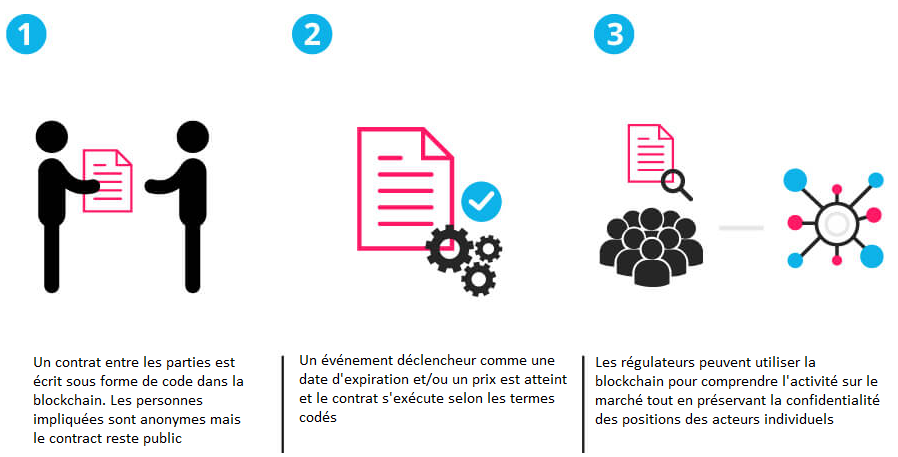
\includegraphics[width=1\textwidth]{contract_smart}
\begin{center}
   \textbf{\underline{Processus d'un smart contract}} \\[1cm]
\end{center}


%%%%%%%%%%%%%% Prêt bancaire %%%%%%%%%%%%%%

     \item \textbf{Faire un prêt! }
    
\hspace{1cm} Les prêts sont limités entre autre dans un même territoire. Vous ne pouvez pas faire des prêts à l'étranger. Mais avec la blockchain c'est bien possible! Blockchain  est décentralisée, donc avoir une plate-forme permettant de faire des prêts entre particuliers de manière transparente et sécurisée. Mais aussi faire des emprunts à l'échelle mondiale. De ce fait un emprunteur en France ne sera pas seulement limité aux préteurs locaux, il pourra accéder aux financements venant des États-Unis, d'Asie ou d'ailleurs. \\

\hspace{1cm} Ce qui signifie que pour les prêteurs il y a plus de possibilités d’investissement. Car ce système permet l’internationalisation du marché du crédit ainsi qu’un accès plus rapide à celui ci par rapport à l’utilisation du système bancaire actuel. Les transactions sont effectuées en quelques secondes ou minutes comparés aux jours d’attente que vous pouvez rencontrer dans le système bancaire actuel. Ceci favorisera aussi la compétition sur les taux d'intérêts.

\end{enumerate}

%%%%%%%%%%%%%% Problème %%%%%%%%%%%%%%
    \subsection{Faiblesses de la blockchain}
\hspace{1cm} Nous pouvons nous demander si c'est une bonne idée d'utiliser la blockchain pour les transferts d’argent. Pour l'utilisation des blockchains nous avons besoin d’un marché de crypto monnaies dans le pays qui envoie et d’un autre marché dans le pays qui reçoit. On a aussi besoin qu’il y ait des échanges dans ces pays et qu’il y en ait suffisamment pour obtenir la liquidité des transferts d’argent. Ce qui pose un vrai problème car non seulement les marchés de crypto monnaies ne sont pas présent partout mais aussi le prix d’une crypto dans un pays n’est pas le même que dans un autre pays. Le manque de liquidité et les décalages de marché sont 2 gros freins à l’utilisation des crypto monnaies pour les envois d’argent.\\

\hspace{1cm} Nous avons aussi des contraintes non négligeables sur l’aspect régulatoire. En effet pour faire es transferts d’argent, il faut une licence dans les pays concernés. Ce qui risque d'amener des coûts exorbitants des licences, plusieurs millions, dans chaque pays qui applique ses propres lois\\

\hspace{1cm} Nous avons aussi le problème de la volatilité de la monnaie si on cherche à transférer de l’argent sur base d’échanges de crypto monnaies. La monnaie est soumise à la loi de l'offre et de la demande, ce qui fait que le prix augmente quand la demande est forte et diminue lorsque la demande est faible. C'est pour ça qu'il est jugé dangereux d'investir dedans. C'est le cas d'un Un investisseur de 32 ans originaire des Émirats arabes unis qui a emprunté 139 000 dollars pour investir dans la crypto-monnaie. Mais il il a perdu 85\% de la somme et doit rembourser 3381 dollars par mois jusqu’en 2021 juste parce que la valeur de ses jetons ont chuté. Ainsi le cours de la monnaie est très instable et évolue de manière imprévisible, en témoignent les fortes fluctuations de son prix ces derniers mois, à des périodes très rapprochées. Le montant perçu lors d'une vente peut varier entre le moment de l'achat et celui de la réception du paiement. Voir \textbf{annexe 3} \\

\hspace{1cm} Nous ne pouvons pas ne pas parler de la sécurité de la blockchain qui est très sécurisée. Nous avons vu,avec notre blockchain, que tout est sécurisé et qu'on passe le Proof of Work. Mais cet aspect est l'une des principales de la technique de la blockchain. Chaque transaction, comme on l'a vu, est inscrite bloc après bloc dans le registre de la cryptomonnaie après avoir été vérifiée par les mineurs, au travers du calcul cryptographique. Et quand quelqu’un détient plus de la moitié de la puissance de calcul,\textbf{51\% de la puissance de calcul de minage} , il a la main sur cette procédure de vérification et peut alors invalider des transactions passées. Ce qui ouvre les portes à une une arnaque appelée la  \textbf{double dépense}. Comment ça fonctionne? Le pirate réalise une double transaction du même montant, au même moment : un achat auprès d'un vendeur et un transfert vers l'un des wallets qu'il contrôle. Il va donc concentrer ses calculs sur la 2ème l'autre côté, le vendeur voit arriver une transaction tout à fait normale et décide donc l’accepter. Le montant est échangé contre un bien que le pirate va directement rapatrier le plus vite possible. Ensuite il diffuse ses propres blocs de vérification, ce qu'il peut faire parce qu'il contrôle plus de 50\% de la puissance de calcul de minage. Et hop la transaction vers le vendeur est annulée au profit de la transaction vers le wallet du pirate. Au final le vendeur ne recevra rien et le pirate y gagne doublement.\\
Malgré la forte sécurité des cryptomonnaie, cette dernière a déjà subit des attaques. C'est le cas de \textbf{Coinche} qui a été victime d'un vol de \textbf{530 millions de dollars de XEM}. Il s'agit du plus grand vol de l’histoire dont a été victime un site d’échange de crypto-monnaies.

%%%%%%%%%%%%%% Conclusion générale %%%%%%%%%%%%%%
\newpage    
\section{Conclusion}

\hspace{1cm} La blockchain est devenue un sujet incontournable cette année. Elle dispose beaucoup d'avantages incontestables en termes de rapidité et de sécurité. Cette technologie est tellement sécurisée que les cyber-criminels, bien vrai qu'ils peuvent pirater les individus, ne pourront jamais  voler vos données, car il est pratiquement impossible de pirater une blockchain tout entier. Et c'est grâce à ce caractère décentralisé, couplé avec sa sécurité et sa transparence que la blockchain pousse les particuliers et les entreprises à l'utiliser sans besoin de faire appel à des intermédiaires ou des frais excessifs . Les seuls frais possibles à payer sont la maintenance et la sécurisation du réseau. Ainsi cette technologie pourrait, non pas remplacer les transactions traditionnelles, mais plutôt les améliorer. Elle permettra de de faciliter les transactions, de les rendre beaucoup plus flexible et accessible pour tous. \\ 

\hspace{1cm} Cependant nous rencontrons plusieurs obstacles sur l'existence et l'utilisation des blockchains. Tout le monde n'est pas du même avis. Nous avons \textbf{Grégory Chenue}, chef de projet Marketing au Crédit Agricole, qui pense je cite "\textit{Tout casser pour remplacer par des systèmes blockchain prendrait beaucoup de temps car on ne part pas de zéro, les infrastructures de réseau sont très complexes}" La complexité du système pause un grand soucis pour les détenteurs des monnaies bancaires et l'instabilité des monnaies virtuelles leur font vraiment peur. \\

\hspace{1cm} Sur le plan de la finance c'est pas encore gagné. Déjà en 2012, la Banque centrale européenne avait défini la monnaie virtuelle comme un type de monnaie numérique non réglementée, émise et généralement contrôlée par ses développeurs, une monnaie utilisée et acceptée par les membres d'une communauté virtuelle spécifique. En 2014, L'autorité bancaire européenne catégorise la monnaie virtuelle de monnaie numérique qui a aucune valeur et qui n'est pas du tout officielle.

\hspace{1cm} Malgré ces divergences il y a de plus en plus d'institutions bancaires qui commencent à s'y intéresser et commencent à réaliser des transactions. Mais pour que la blockchain soit officiellement opérationnelle dans ces institutions, il faudra dans un premier temps réguler les monnaies virtuelles. Et ensuite trouver une solution pour gérer la fluctuation de celles-ci. Il faudra aussi sensibiliser le grand public qui est encore peu familiarisé avec cette monnaie virtuelle, dont le fonctionnement tranche encore avec les devises monétaires habituelles. Il est donc assez difficile d’évaluer l’importance que pourrait pourrait prendre la blockchain dans les années à venir.\\

%%%%%%%%%%%%%% Webo %%%%%%%%%%%%%%
\newpage
\section{Webographie}

\begin{itemize}
    \item \url{https://www.journaldunet.com/economie/finance/1179949-blockchain-publique\\-privee-consortium-quelles-differences/}
    \\
    \item \url{https://bitcoin.org/bitcoin.pdf}
    \\
    \item \url{https://www.lesechos.fr/17/10/2017/lesechos.fr/030736112801_blockchain---\\les-banques-multiplient-les-projets-d-exploration.htm}
    \\
    \item \url{http://www.revue-banque.fr/management-fonctions-supports/article/blockchain-dans-banque-quels-developpements-pour-a}
    \\
    \item \url{https://www.journaldunet.com/economie/finance/1179675-la-bataille-secrete-\\des-banques-pour-mettre-la-main-sur-la-blockchain/}
     \\
    \item \url{https://www.andlil.com/fiscalite-bitcoin-crypto-monnaies-202183.html}
     \\
    \item \url{http://www.viatys.com/lere-blockchain-technologie-a-facteur-dacceleration\\-dobsolescence-innovations-actuelles/}
     \\
    \item \url{https://www.begeek.fr/guide-bases-minage-de-bitcoin-ethereum-litecoin-autres\\-crypto-monnaies-247026}
     \\
    \item \url{https://blockchainfrance.net/2016/08/17/quels-impacts-de-la-blockchain-sur\\-les-banques/}
     \\
    \item \url{https://fr.investing.com/analysis/la-regularisation-des-cryptomonnaies-ne\\-saurait-tarder-200218948}
\end{itemize}
\quad

Le lien vers mon GitHub qui contient le code en latex ainsi qu'une version pdf :\\ 
\url{https://github.com/sokhnaSow/Memoire_M2_Miage/tree/master/Presentation-Memoire}

\newpage
\section{Annexes}

\textbf{Annexe 1}\\
\begin{center}
    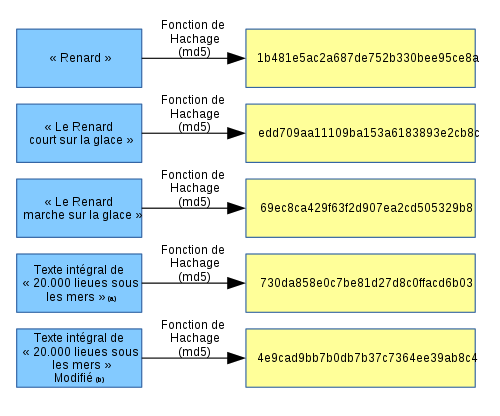
\includegraphics[width=1.2\textwidth]{hashage}
\end{center}

\newpage
\textbf{Annexe 2}\\
\begin{center}
   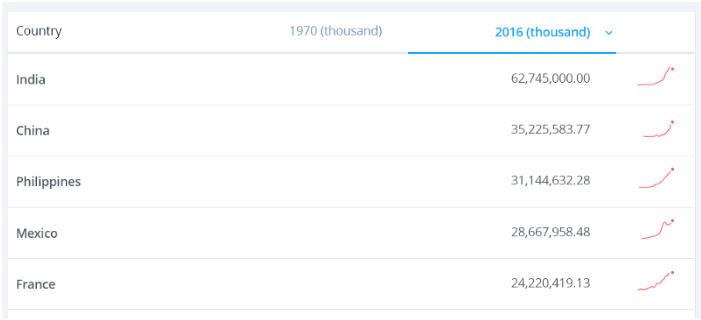
\includegraphics[width=1\textwidth]{transfert_pays.png}
\end{center}

\newpage
\textbf{Annexe 3}\\
\begin{center}
    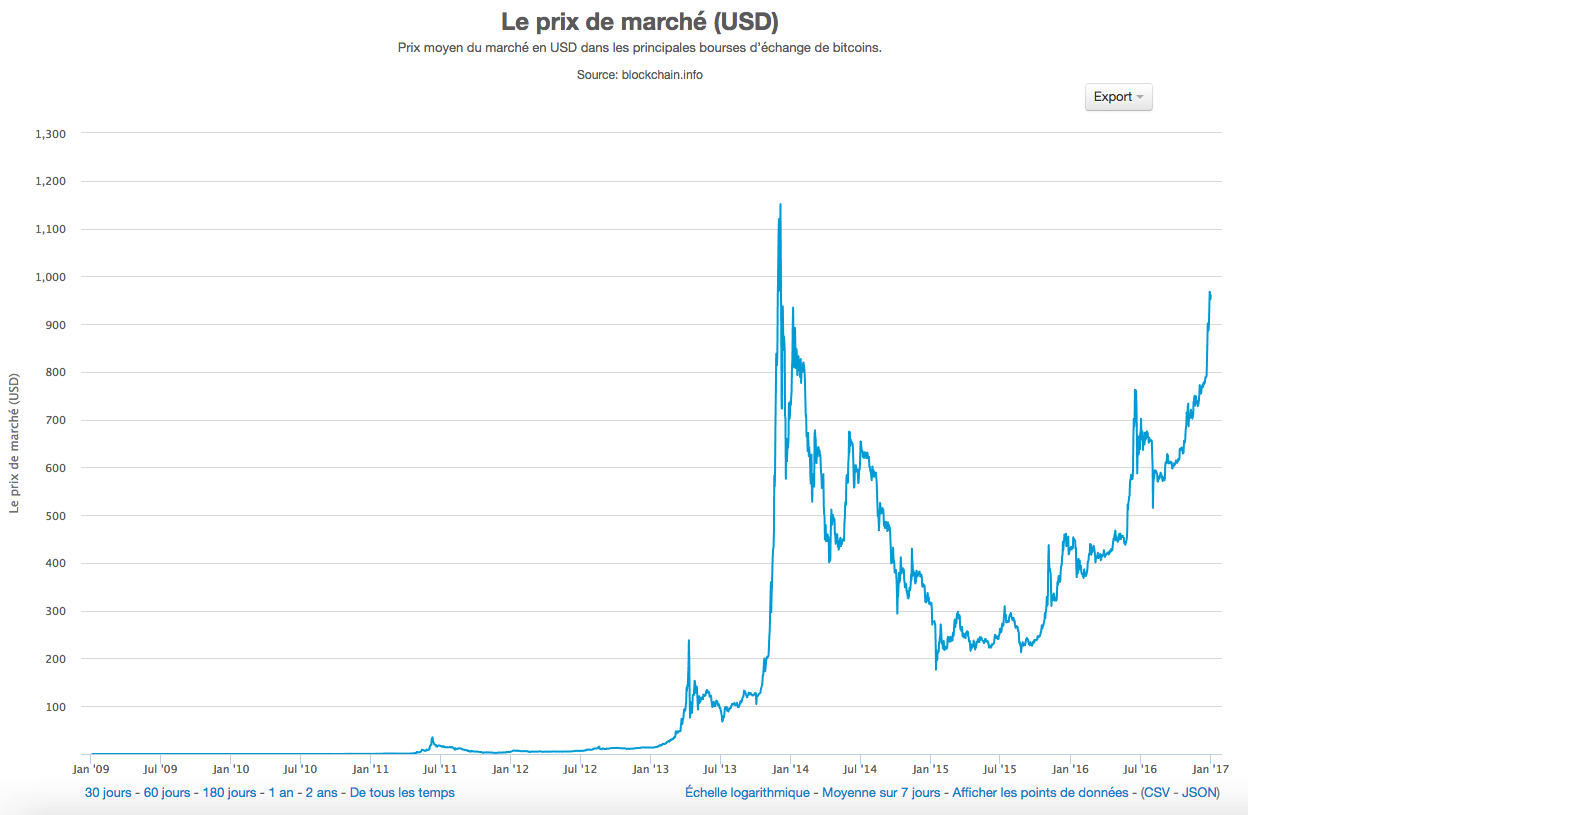
\includegraphics[width=1.3\textwidth]{courbeBTC}
\end{center}


\end{document}  